% Gemini theme
% https://github.com/anishathalye/gemini

\documentclass[final]{beamer}

% ====================
% Packages
% ====================

\usepackage[T1]{fontenc}
\usepackage{lmodern}
%\usepackage[size=custom,width=120,height=72,scale=1.0]{beamerposter}
\usepackage[size=a0,scale=1.1]{beamerposter}
\usetheme{gemini}
\usecolortheme{mit}
\usepackage{graphicx}
\usepackage{booktabs}
\usepackage{tikz}
\usepackage{pgfplots}
\usepackage[caption=false,font=small]{subfig}
%\usepackage{subcaption}
% ====================
% Lengths
% ====================

% If you have N columns, choose \sepwidth and \colwidth such that
% (N+1)*\sepwidth + N*\colwidth = \paperwidth
\newlength{\sepwidth}
\newlength{\leftcolwidth}
\newlength{\maincolwidth}
\newlength{\rightcolwidth}
\setlength{\sepwidth}{0.025\paperwidth}
\setlength{\maincolwidth}{0.3\paperwidth}
\setlength{\leftcolwidth}{0.3\paperwidth}
\setlength{\rightcolwidth}{0.3\paperwidth}

\newcommand{\separatorcolumn}{\begin{column}{\sepwidth}\end{column}}

% ====================
% Title
% ====================

\title{Stopping Silent Sneaks: Defending against Malicious Mixes through Topological Engineering}

\author{\textbf{Xinshu Ma} \inst{1} \and Florentin Rochet \inst{2} \and Tariq
 Elahi \inst{1}}

\institute[shortinst]{\inst{1} \Large University of Edinburgh
\samelineand \inst{2} University of Namur}
%\samelineand \inst{2} U.S. Naval
 %Research Lab \samelineand \inst{3} Princeton University}

% ====================
% Body
% ====================

\begin{document}

\begin{frame}[t]
\begin{columns}[t]
\separatorcolumn

\begin{column}{\leftcolwidth}

%  \begin{block}{Goals}
%    Mitigate private infrastructure threats due to adversarial resources (META)
%    
%    \textbf{Reduce the end-to-end compromised traffic in mixnets while optimising tradeoff between security and performance.}
%    
%%    \begin{itemize}
%%      \item \textbf{Focus on the impact of topological construction on mixnets
%%      Investigate topological, no topology right now.
%%      }
%%      \item \textbf{Optimise tradeoff between security and performance
%%      Balance the tradeoffs between security and performance}
%%      \item \textbf{Reduce end-to-end compromise
%%      %Optimal path selection for further improvement on security.
%%      }
%%    \end{itemize}
%
%  \end{block}

\begin{block}{Problem}

\heading{Trustworthy Mixnet Construction from Untrusted Resources}

\begin{center}
  \begin{figure}
    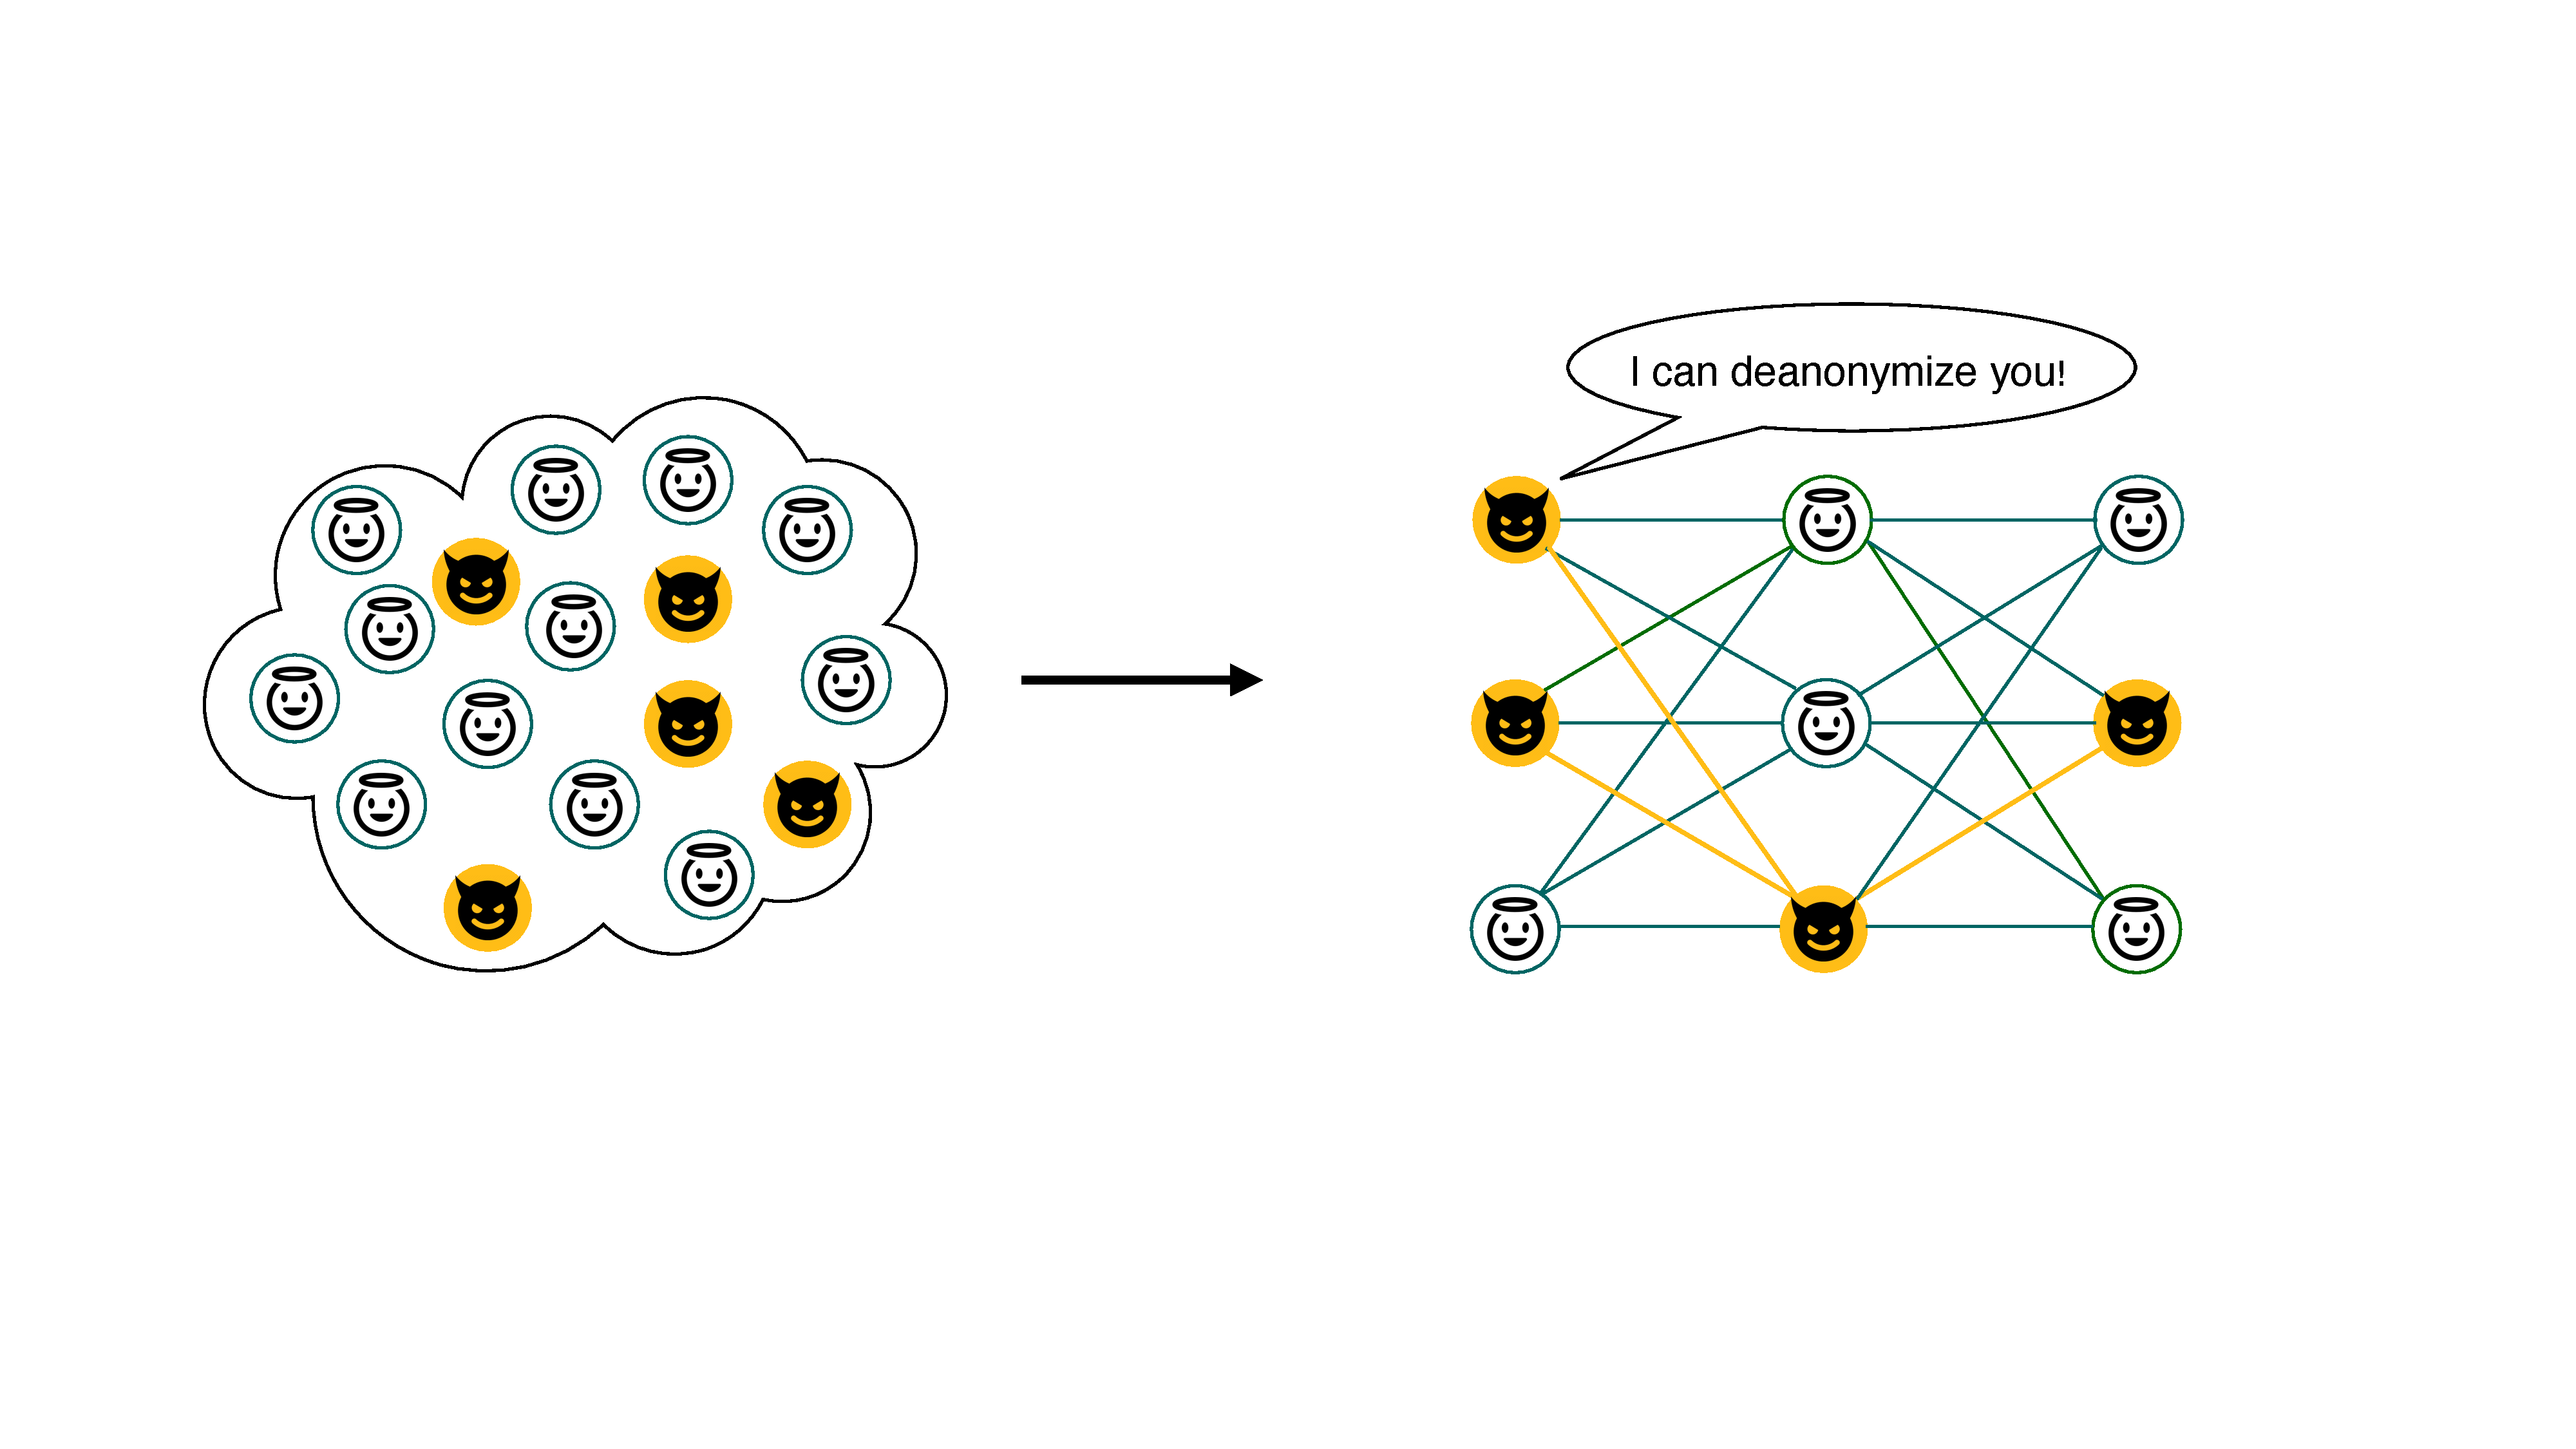
\includegraphics[width=\rightcolwidth]{images/problem_overview.pdf}
    \caption{\textbf{Anytrust assumption} might break in the real world: users suffer from \textbf{end-to-end compromise} and \textbf{client enumeration} by passive adversary.}
  \end{figure}
  
  \vspace{1cm}

    \begin{figure}
    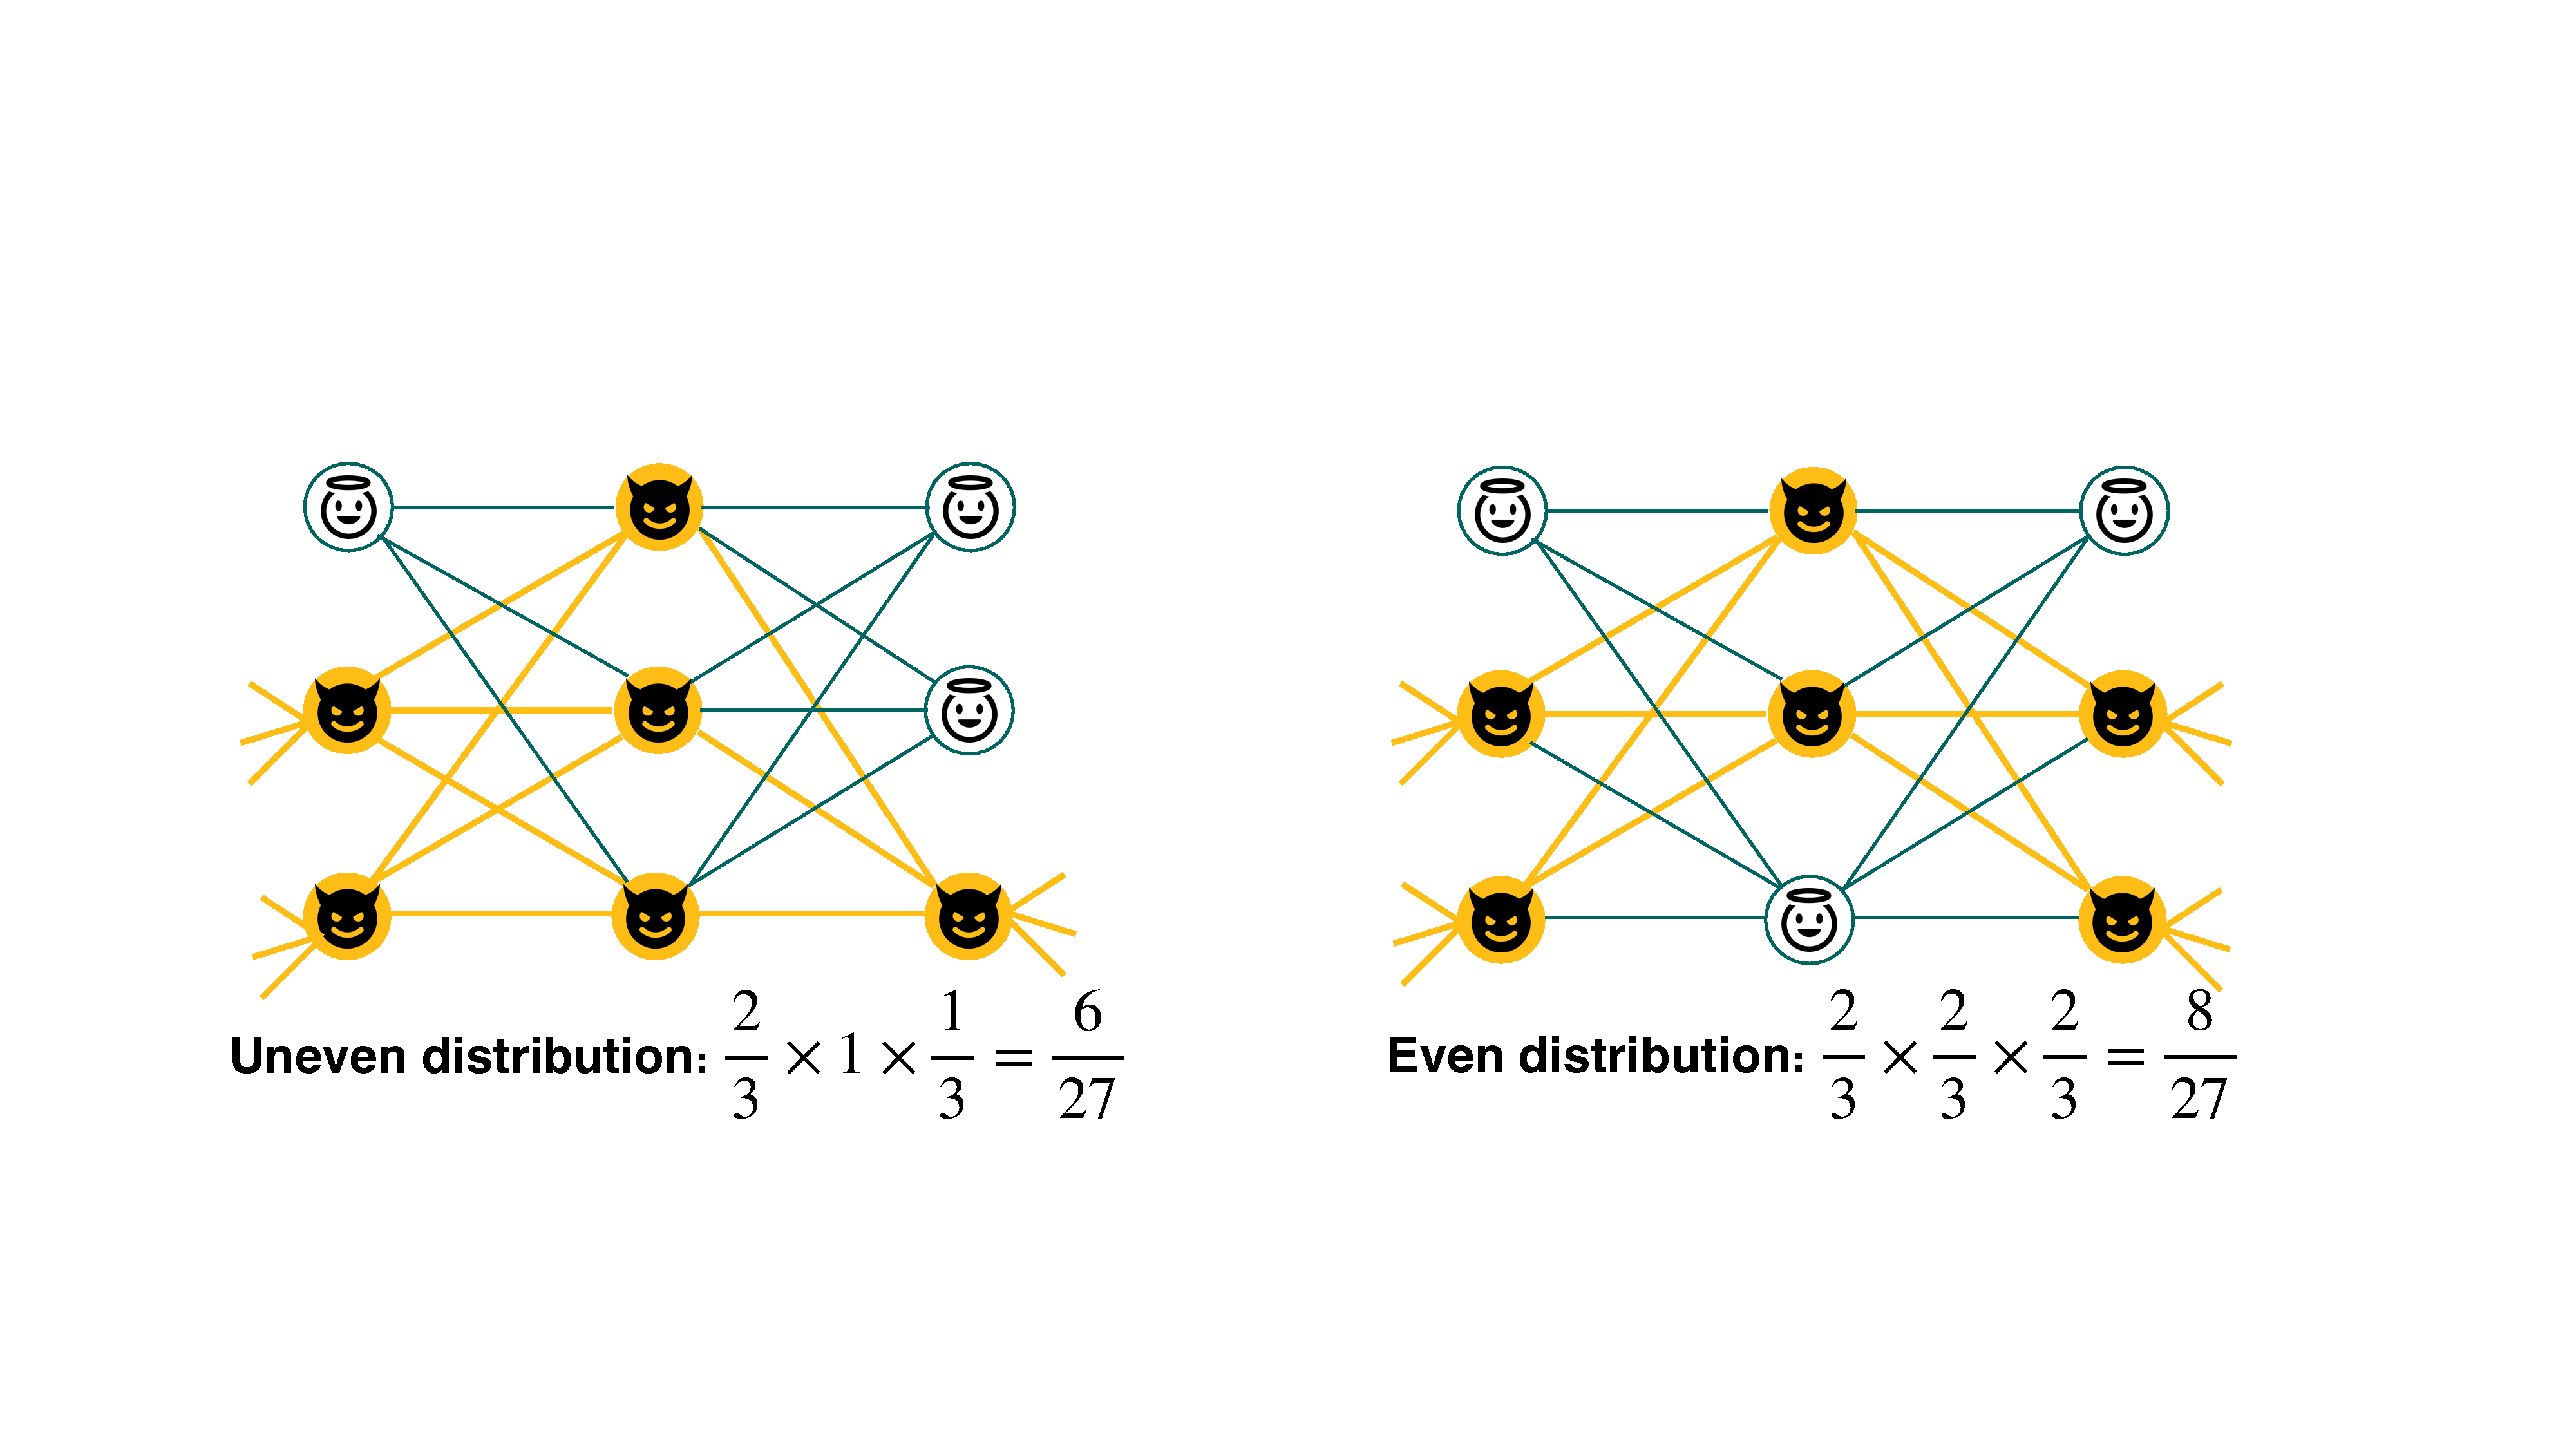
\includegraphics[width=\rightcolwidth]{images/problem_max.pdf}
    \caption{Adversary \textbf{maximizes} the compromised rate by achieving even distribution.}
  \end{figure}
  
  \vspace{1cm}
  
    \begin{figure}
    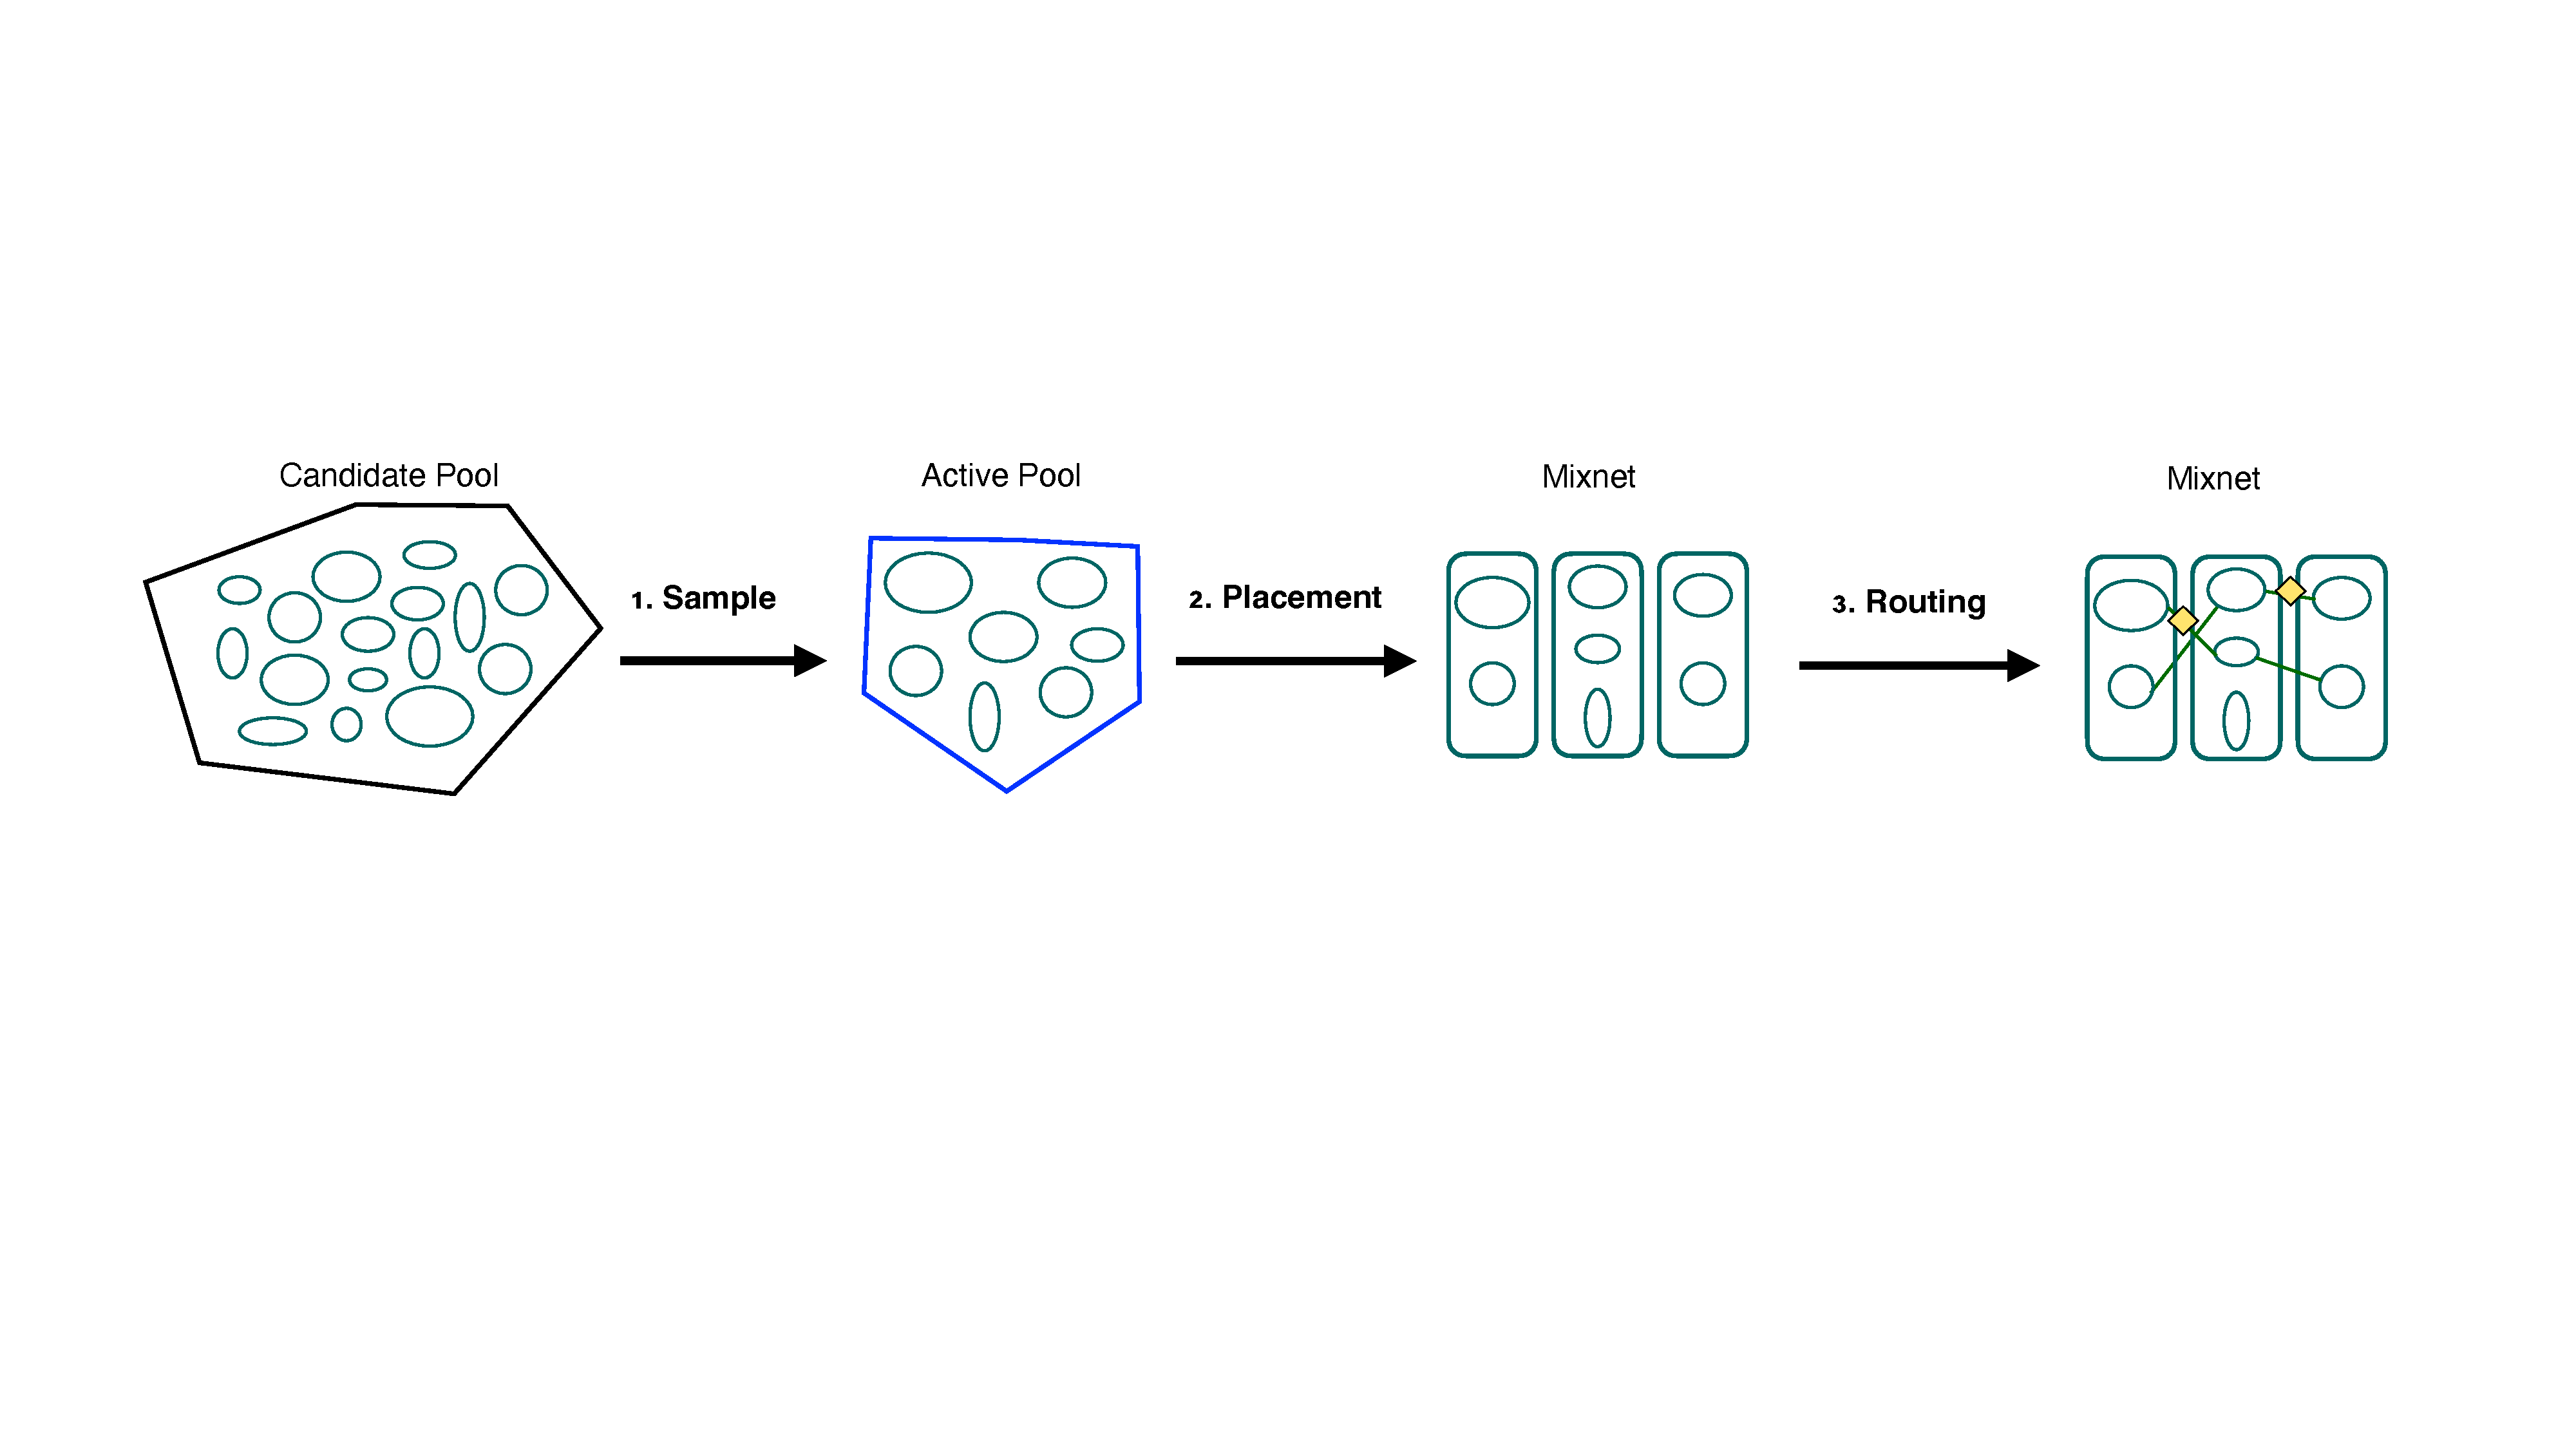
\includegraphics[width=\rightcolwidth]{images/problem_model.pdf}
    \caption{Mixnet construction model: 3-stage process.}
  \end{figure}
    \end{center}
\end{block}

\begin{block}{}
\heading{Example of Adversary's Manipulation}
  \begin{figure}
    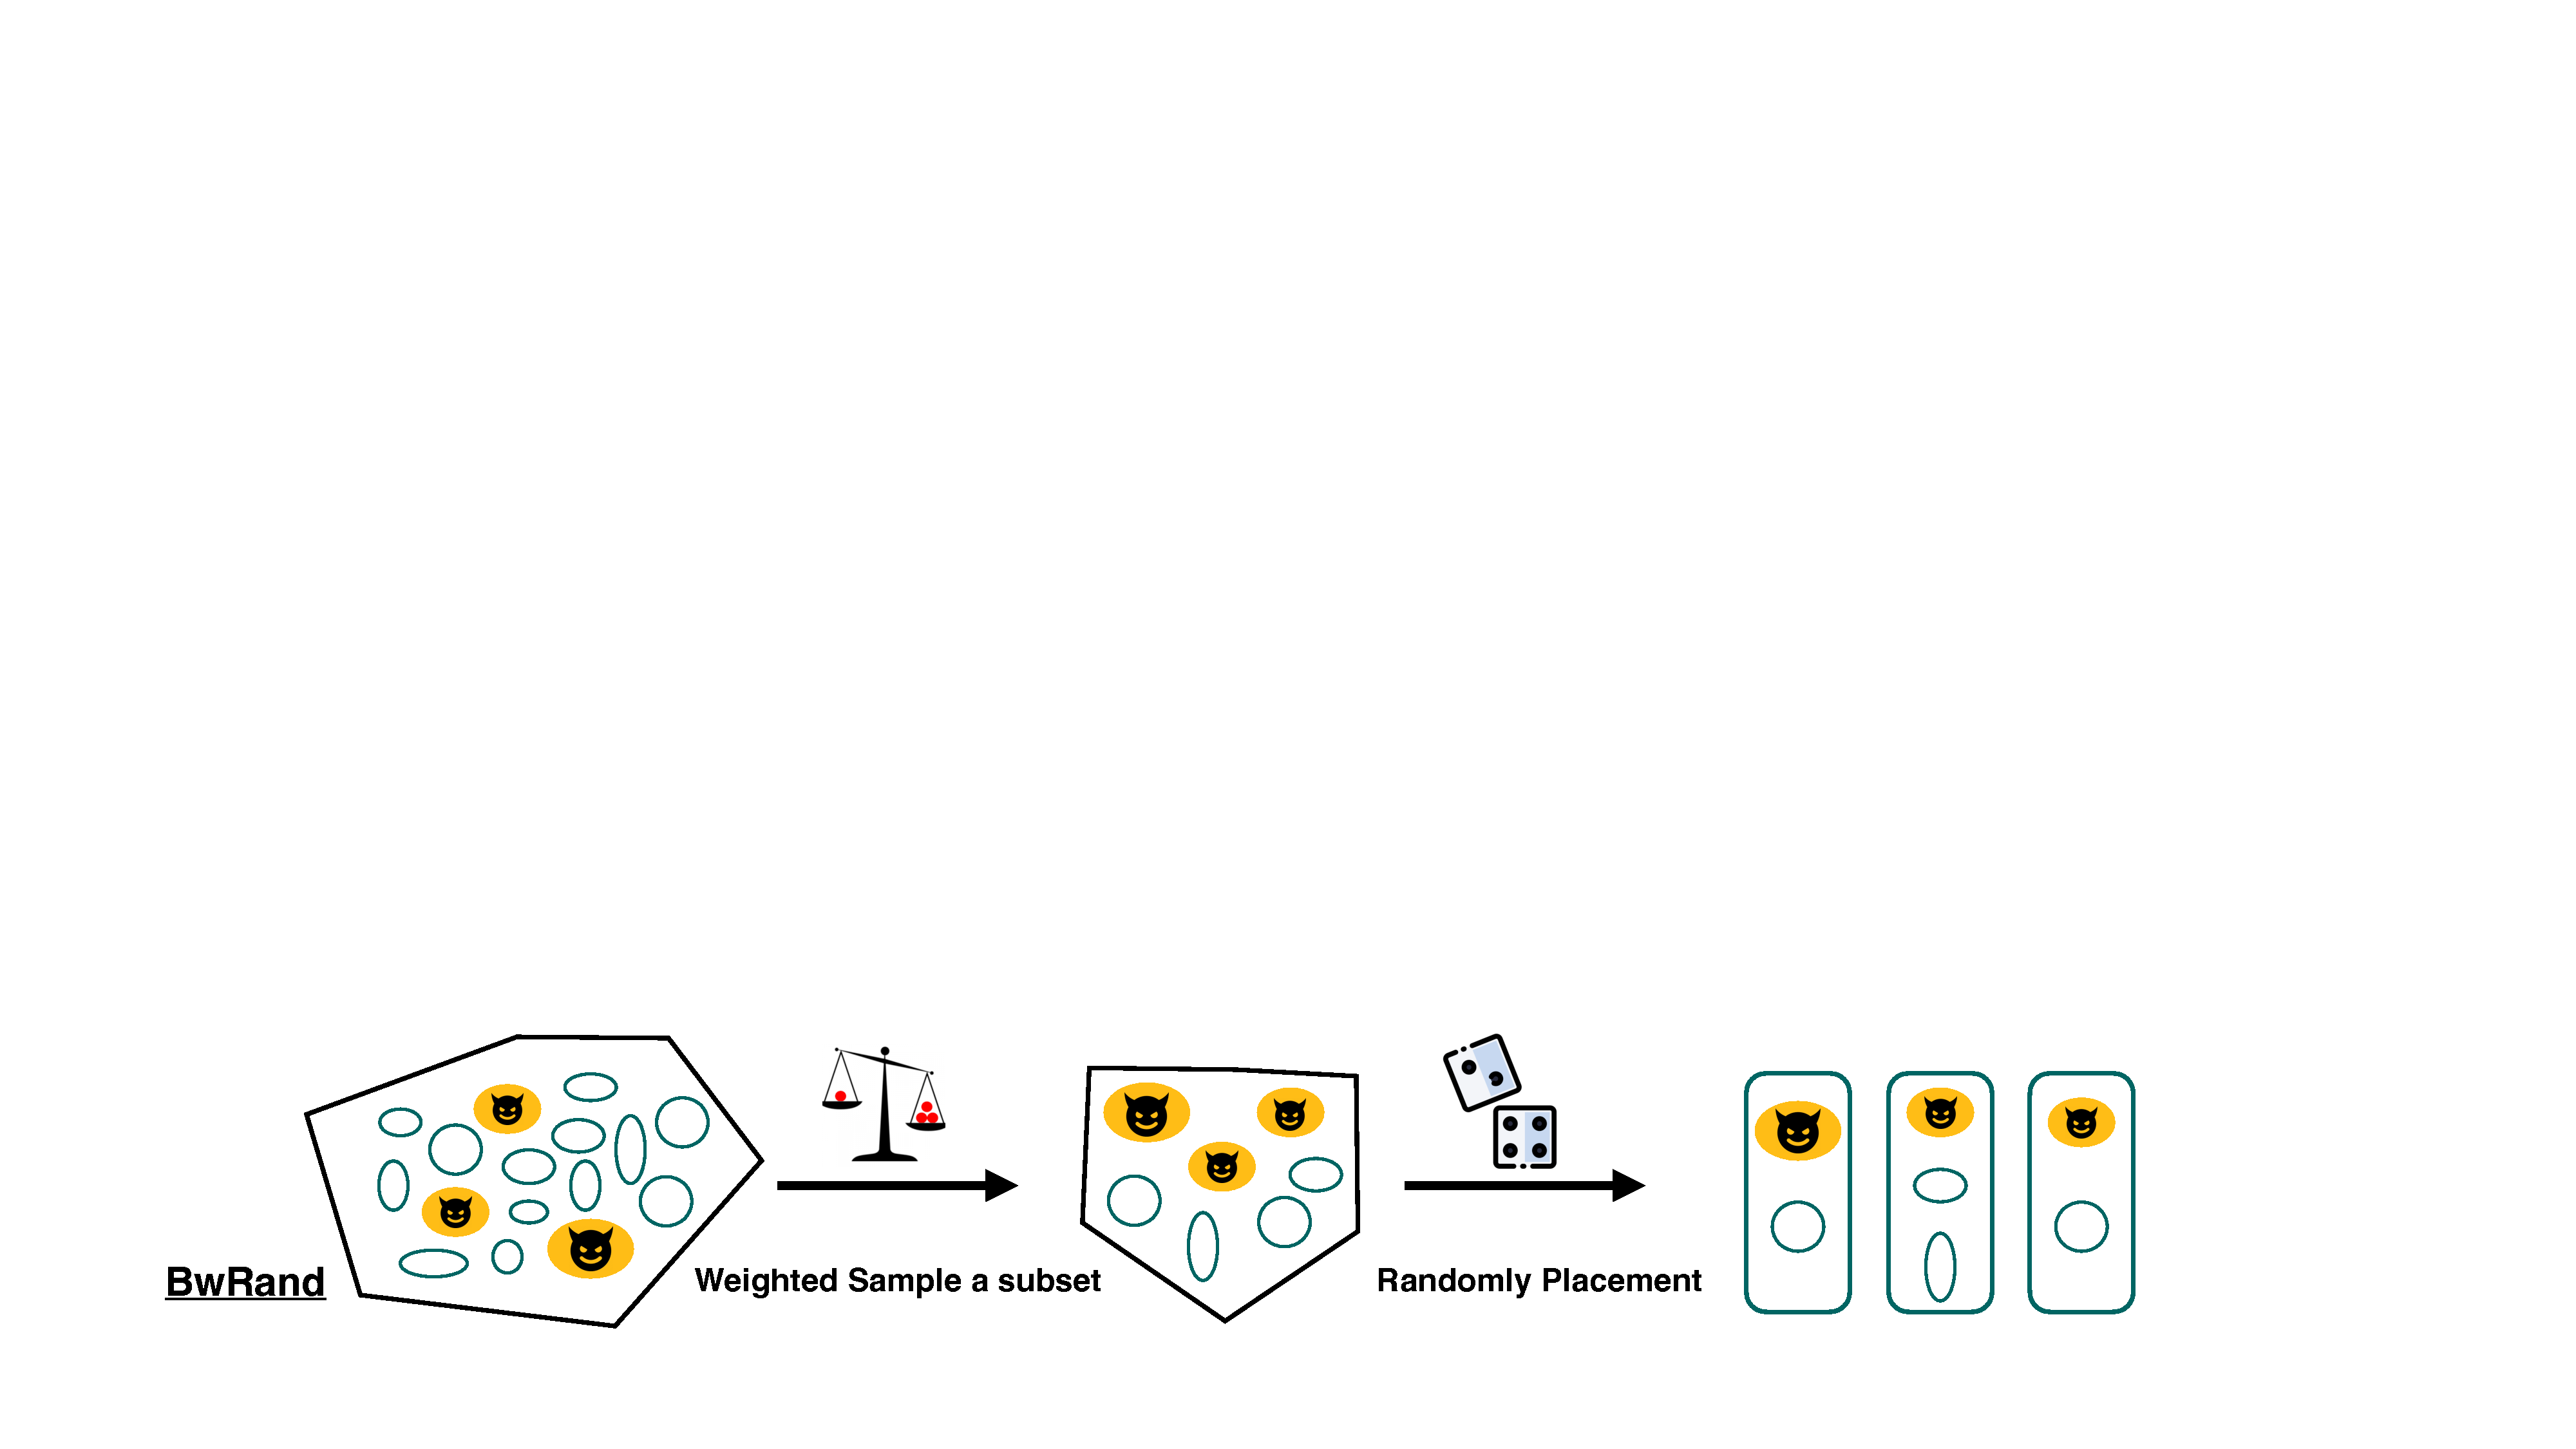
\includegraphics[width=\rightcolwidth]{images/problem_eg.pdf}
    \caption{Adversary can compromise more than $10\%$ of total traffic with $\alpha=0.2$ resources by manipulating mixes' bandwidth.}
  \end{figure}
\end{block}


  \begin{minipage}[t]{0.32\rightcolwidth}
   \begin{figure}
   \centering
    
\includegraphics[width=0.8\textwidth]{images/UoE-logo.png}
  \end{figure}
  \end{minipage}
  \hfil
  \begin{minipage}[t]{0.32\rightcolwidth}

  \begin{figure}
    \centering
    
\includegraphics[width=0.8\textwidth]{images/unamur-logo.jpeg}
  \end{figure}
  \end{minipage}
  \hfill
  \begin{minipage}[t]{0.33\rightcolwidth}
\vspace{-1cm}
   \begin{figure}
     \centering
      
\includegraphics[width=0.8\textwidth]{images/REPHRAIN-logo.pdf}
  \end{figure}
  \end{minipage}


%  \begin{block}{Code availability}
%    \begin{center}
%      See me on github!\\
%      https://github.com/CLAPS-CCS2020
%      \begin{figure}
%        \centering
%      
\includegraphics[scale=0.6]{images/githubicon.png}
%      \end{figure}
%      \vspace{-0.7cm}
%    \end{center}
%  \end{block}
%    \begin{center}
%      \vspace{5cm}
%      \begin{figure}
%        
\includegraphics{images/tor_logo.png}
%      \end{figure}
%    \end{center}
\end{column}


\separatorcolumn

\begin{column}{\maincolwidth}

%  \begin{alertblock}{Evaluation Framework}
%
%  \begin{center}
%    \heading{A generic framework to reason on mixnet topological construction}
%  \end{center}
%    
%    \begin{minipage}[t]{0.31\maincolwidth}
%      \begin{center}
%      \heading{Mitigate Adversary's Manipulation} 
%       \begin{itemize}
%         \item Establish a construction algorithm that limits the adversary's advantage
%         \item Quantify the advantage getting from adversarial manipulation
%       \end{itemize}
%     \end{center}
%    \end{minipage}
%    \begin{minipage}[t]{0.31\maincolwidth}
%      \begin{center}
%      \heading{Bound Users' Exposure to Malicious Mixes} 
%       \begin{itemize}
%         \item Establish guard design in mixnet layered routing.
%         \item Quantify users' guard exposure rate
%       \end{itemize}
%     \end{center}
%    \end{minipage}
%    \begin{minipage}[t]{0.31\maincolwidth}
%      \begin{center}
%      \heading{Achieve Sustainable Performance} 
%       \begin{itemize}
%         \item Design sampling and placement strategies.
%         \item Quantify the overhead of message processing and mixnet construction
%       \end{itemize}
%     \end{center}
%    \end{minipage}
%  \end{alertblock}
% \vspace{1cm}

\begin{alertblock}{Results-A Balance between Security and Performance}
\end{alertblock}

 \begin{alertblock}{Results -- Security, Performance, and Efficiency}
    \begin{minipage}[t]{0.95\maincolwidth}
      \vspace{-1cm}
      \begin{figure}[t!]
        \centering
        \subfloat[h=0.35]{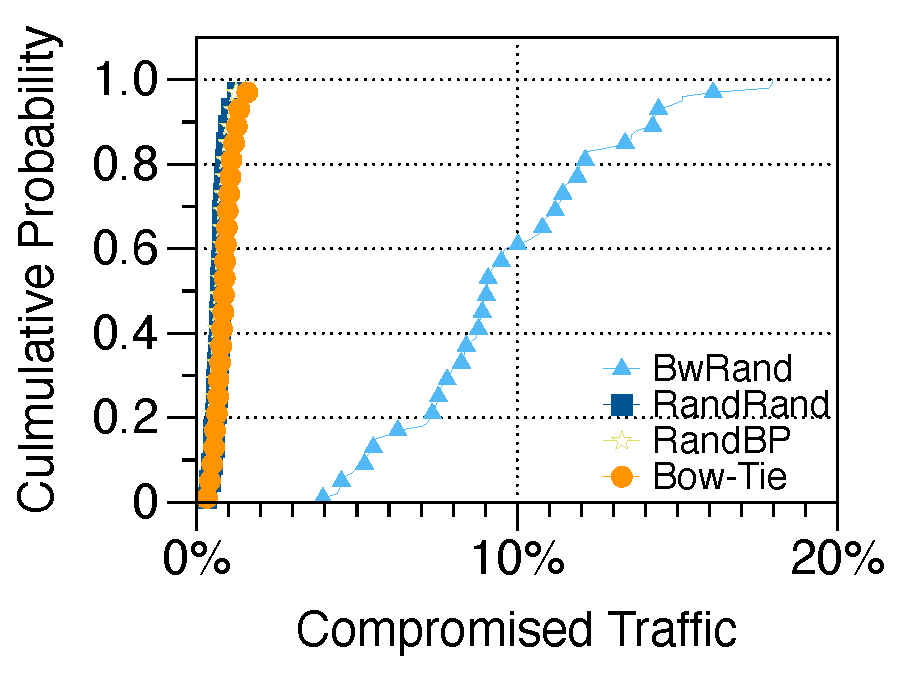
\includegraphics[width=0.33\textwidth]{images/best_bw_35.pdf}}
        \subfloat[h=0.55]{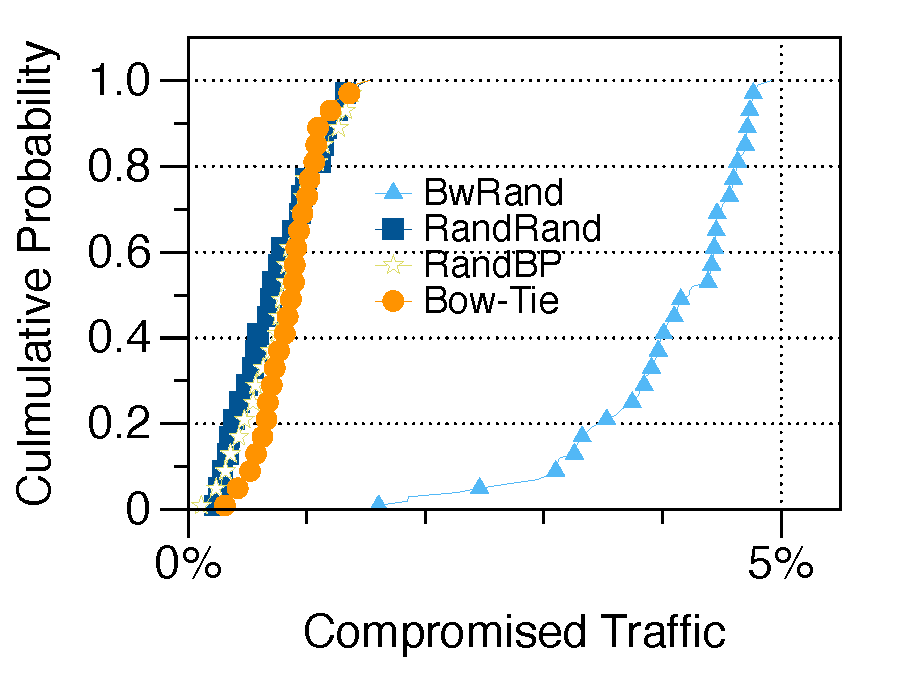
\includegraphics[width=0.33\textwidth]{images/best_bw_55.pdf}}
        \subfloat[h=0.75]{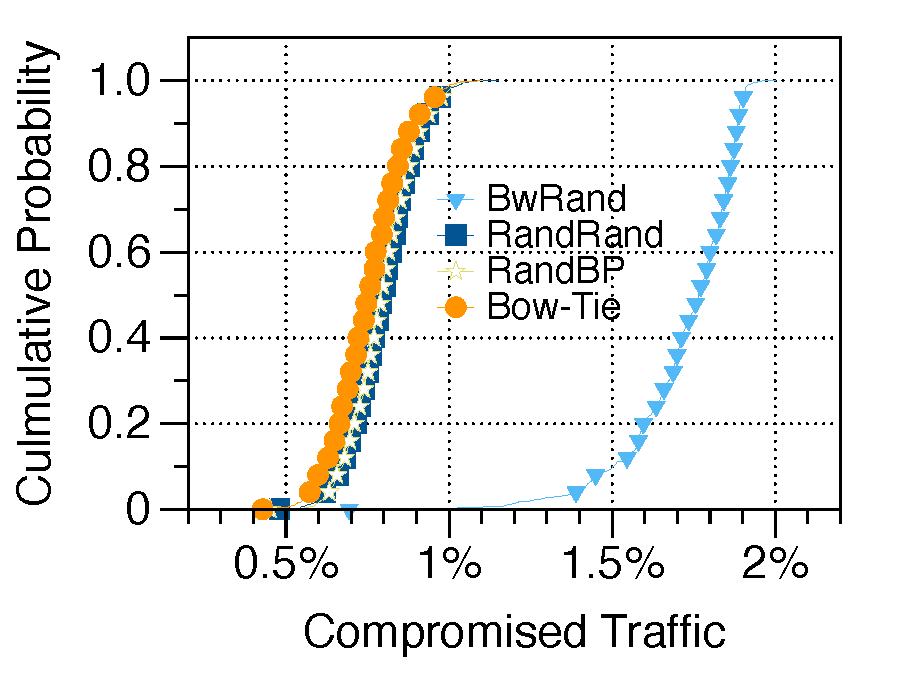
\includegraphics[width=0.33\textwidth]{images/best_bw_75.pdf}}
    \caption{Fully compromised rate versus bandwidth per injected malicious node, as a bandwidth budget of 
    $2280$ MBps is evenly distributed over a varying number of malicious mix nodes, for each mixnet 
    construction strategy. $h$ denotes the threshold at sampling step.}
      \end{figure}
      \vspace{1cm}
\begin{figure}[t!]
    \centering
    \subfloat[No guard]{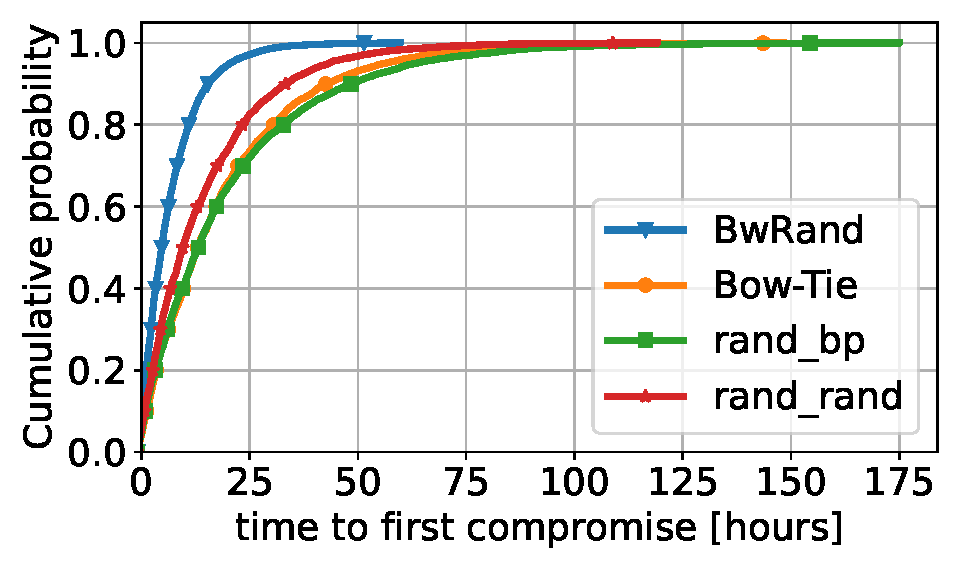
\includegraphics[width=0.33\textwidth]{images/ttfb_static_simple.pdf}}
    \subfloat[With guard]{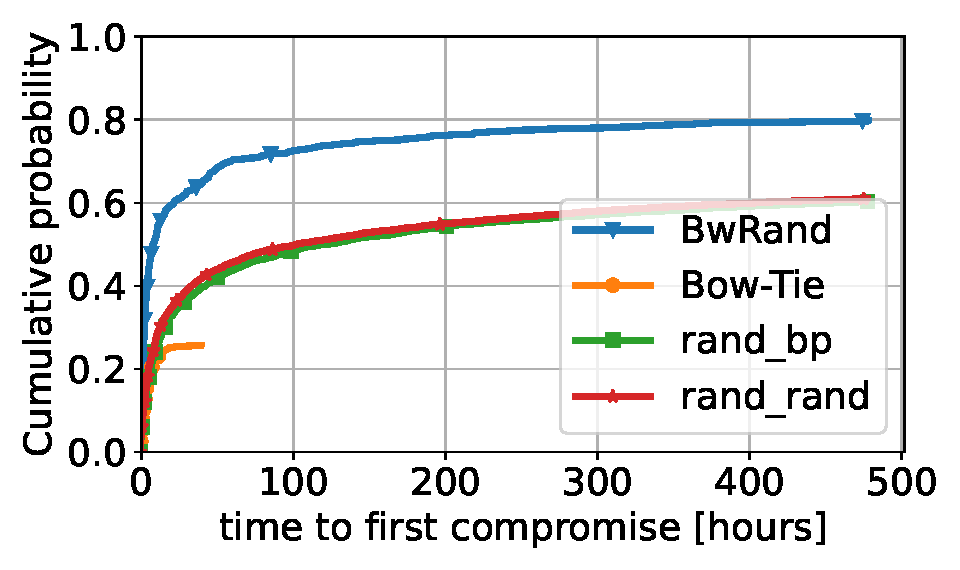
\includegraphics[width=0.33\textwidth]{images/ttfb_static_simple_withguard.pdf}}
    \subfloat[Individual Risks]{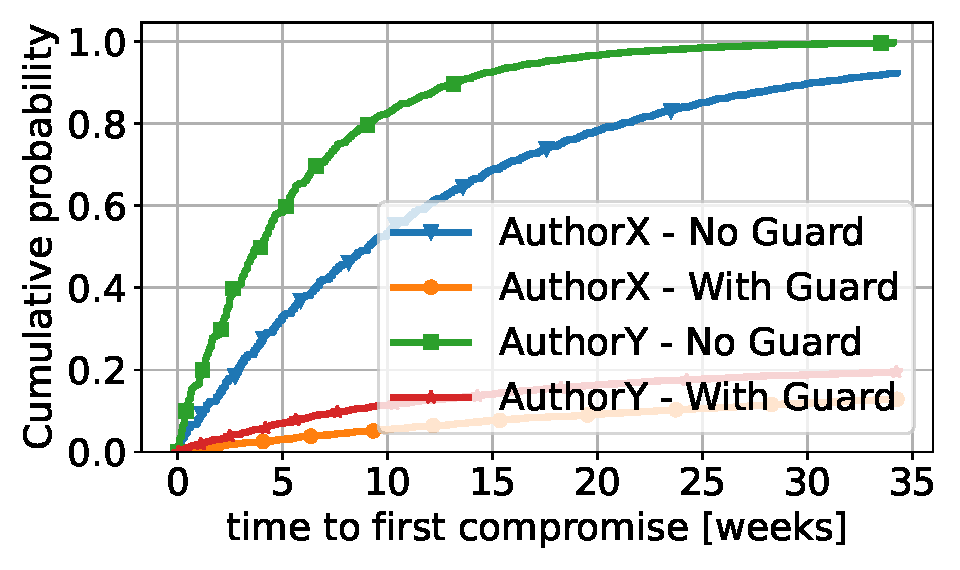
\includegraphics[width=0.33\textwidth]{images/ttfb_email_authors.pdf}}
	%\vspace{-1em}
    \caption{Average time to fall into a fully compromised route for the clients. 
    Figure (a) shows insufficient security if only applying topological construction algorithms. 
    Figure (b) shows discrepancies when our guard proposal is
used for different mixnet topological construction algorithms. 
Figure (c) shows differences when users communicate with different patterns .}
    \label{fig:placement}
\end{figure}
\vspace{1cm}
\begin{figure}[t!]
    \centering
    \subfloat[Bw-weighted path selection]{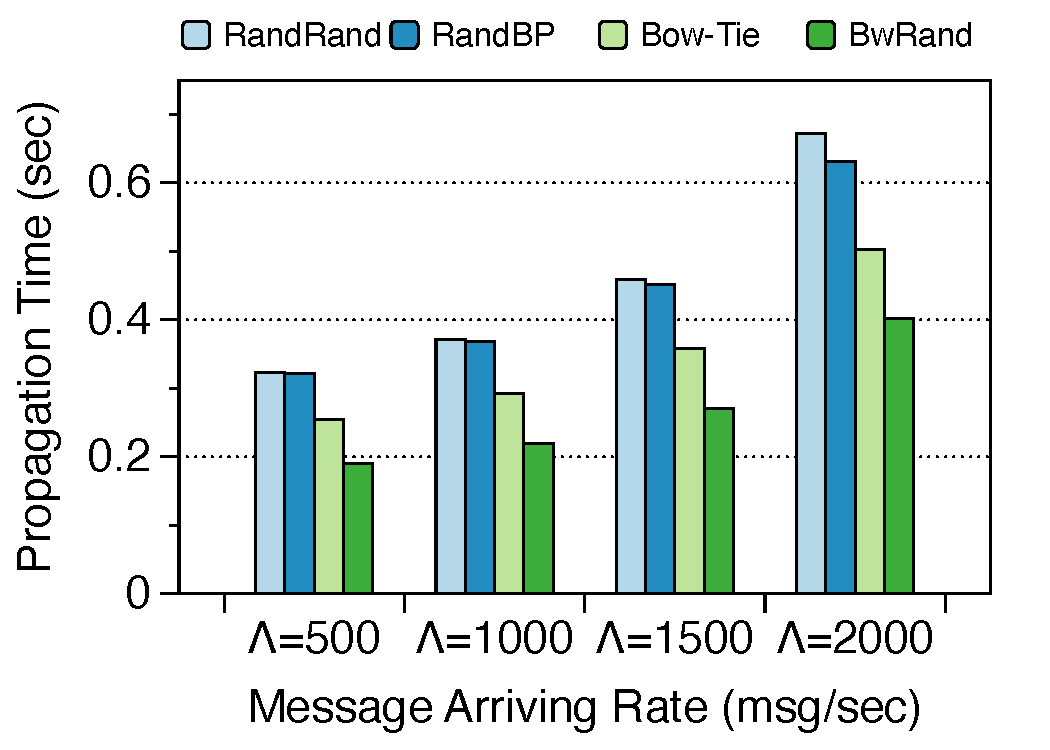
\includegraphics[width=0.33\textwidth]{images/waittime_bw.pdf}}
    \subfloat[Random path selection]{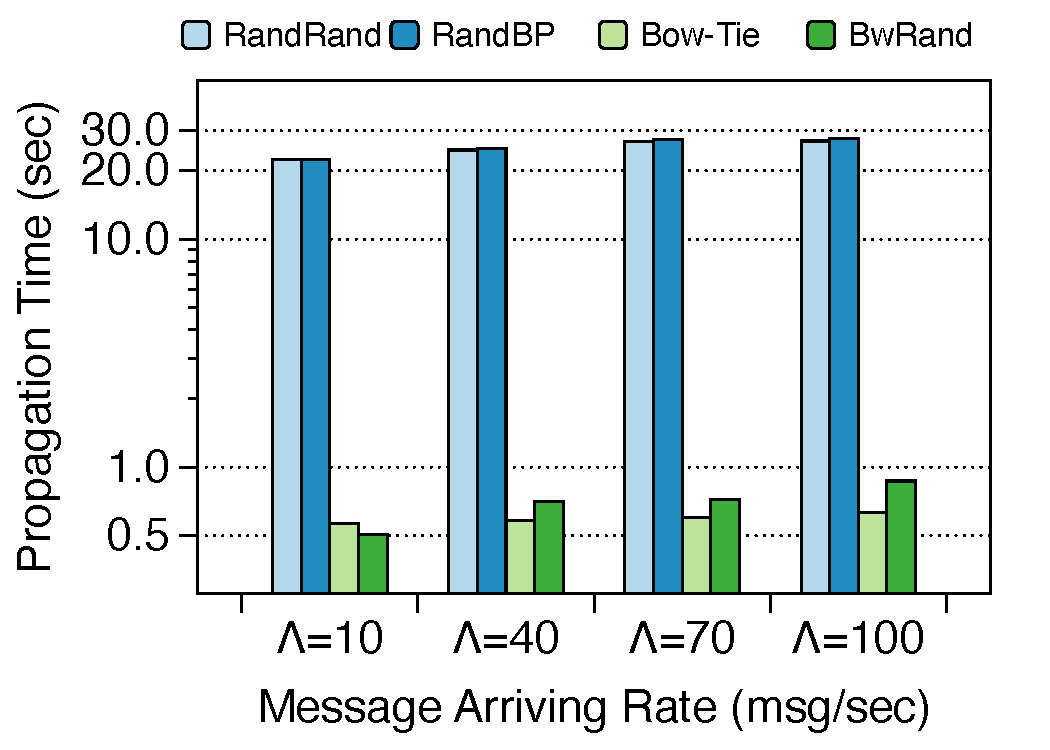
\includegraphics[width=0.33\textwidth]{images/waittime_rand.pdf}}
    \subfloat[Runtime per iteration]{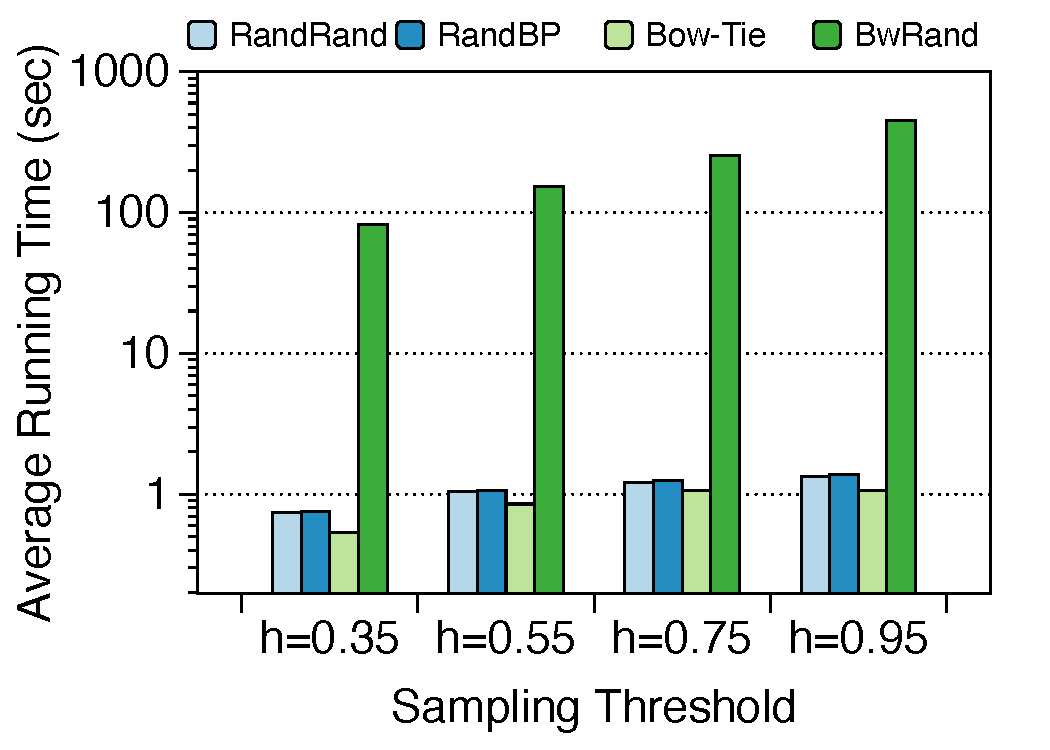
\includegraphics[width=0.33\textwidth]{images/Runtime.pdf}}
%	\vspace{-1em}
    \caption{Propagation time and algorithm runtime.
       \vspace{0em}}
    \label{fig:placement}
\end{figure}
    \end{minipage}
%    \hfill
    
%    \begin{minipage}[t]{0.04\maincolwidth}
%    \end{minipage}
%.   \hfill


%.   comment the minipage to remove the descriptions
%    \begin{minipage}[t]{0.23\maincolwidth}
%          \begin{center}
%      \heading{Security Evaluation 1: \\Fully compromised Traffic} 
%       \begin{itemize}
%         \item The fraction of traffic that are routing via fully compromised paths.
%         %\item The fraction of sampled candidate mixes goes up, the adversary observes less traffic (BwRand).
%         \item The adversary achieves much higher fully compromised rate if the mixnet is constructed by BwRand.
%         \item The fraction of sampled mixes goes up, the adversary observes less traffic of the total.
%       \end{itemize}
%     \end{center}
%
%       
%          \begin{center}
%      \heading{Security Evaluation 2: \\Time to first compromise} 
%       \begin{itemize}
%       	 \item Expected time for the users to choose a fully compromised route.
%	\item With guards, users' security is further improved.
%	%\item Bow-Tie carefully tries to minimize client?s exposure to different guards.
%       \end{itemize}
%     \end{center}
%      
%         \begin{center}
%      \heading{Performance Evaluation: \\Average propogation time} 
%       \begin{itemize}
%         %\item The expected latency, no matter what algorithm, is pretty low with bw-weighted path selection.
%         \item The average time it takes in average to process the message in three layers.
%         \item Bw-PS method handles much more throughput within fixed period of time.
%       \end{itemize}
%     \end{center}
%     
%              \begin{center}
%      \heading{Efficiency Evaluation: \\Algorithm runtime} 
%       \begin{itemize}
%         \item The time it takes to construct a mixnet.
%         \item BwRand consumes highest time while Bow-Tie is the fastest algorithm.
%       \end{itemize}
%     \end{center}
%     
%    \end{minipage}
  
  \end{alertblock}
\end{column}

\separatorcolumn

\begin{column}{\rightcolwidth}

  \begin{block}{Design}
  \heading{Challenges}
  \begin{enumerate}
    \item An adversary's manipulation is hard to detect.
    \item An adversary can perform client enumeration at a low cost.
    \item Tolerating nodes churn.
    \item Performance bottleneck comes from the layer with lowest capacity.
  \end{enumerate}
      
    \heading{Our Approach}
    \begin{enumerate}
    \item Contradictory requirements creates challenges for even distribution.
    \item Guard layer mitigates the risk of client enumeration.
    \item Stability tracking and network maintenance design.
    \item Bin-packing placement to reach even layer capacity.
    \end{enumerate}
    
    \heading{Bow-Tie: High-level Overview}
    \begin{figure}[t]
    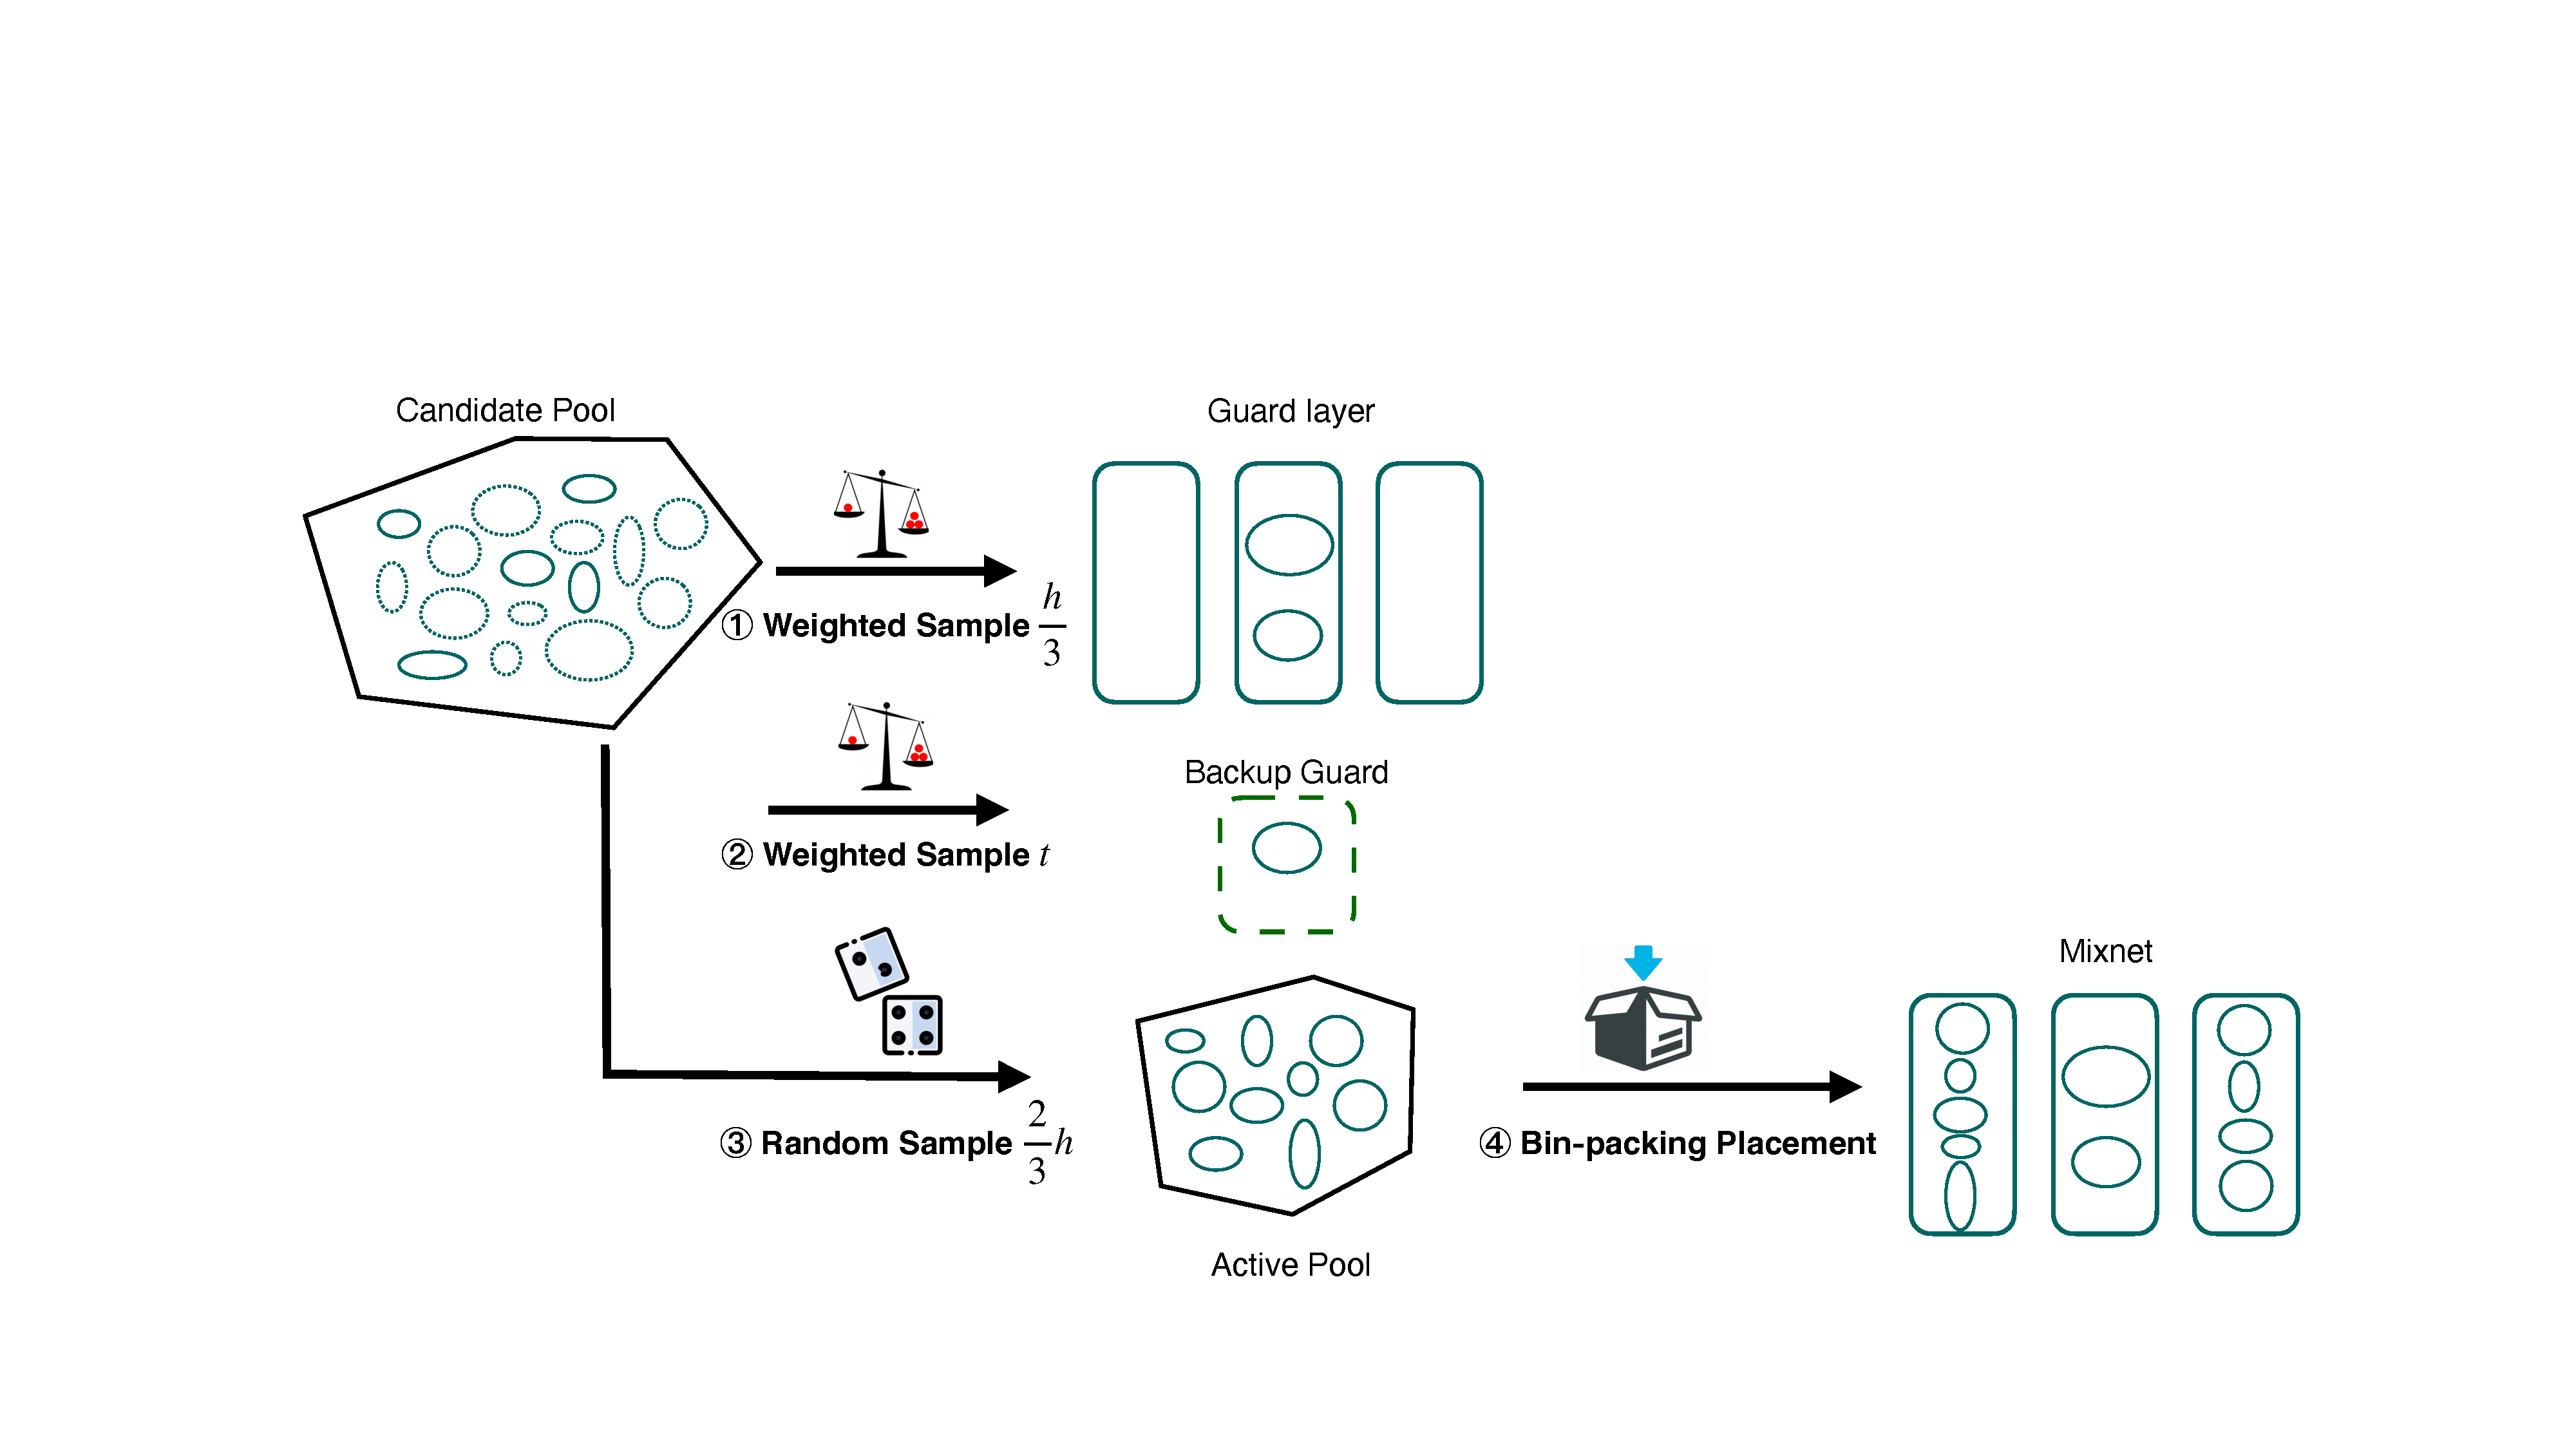
\includegraphics[width=0.95\rightcolwidth]{images/bowtie_init.pdf}
    \caption{Mixnet Initialization}
    \end{figure}
%     \vspace{1cm}
%    \begin{figure}[t]
%    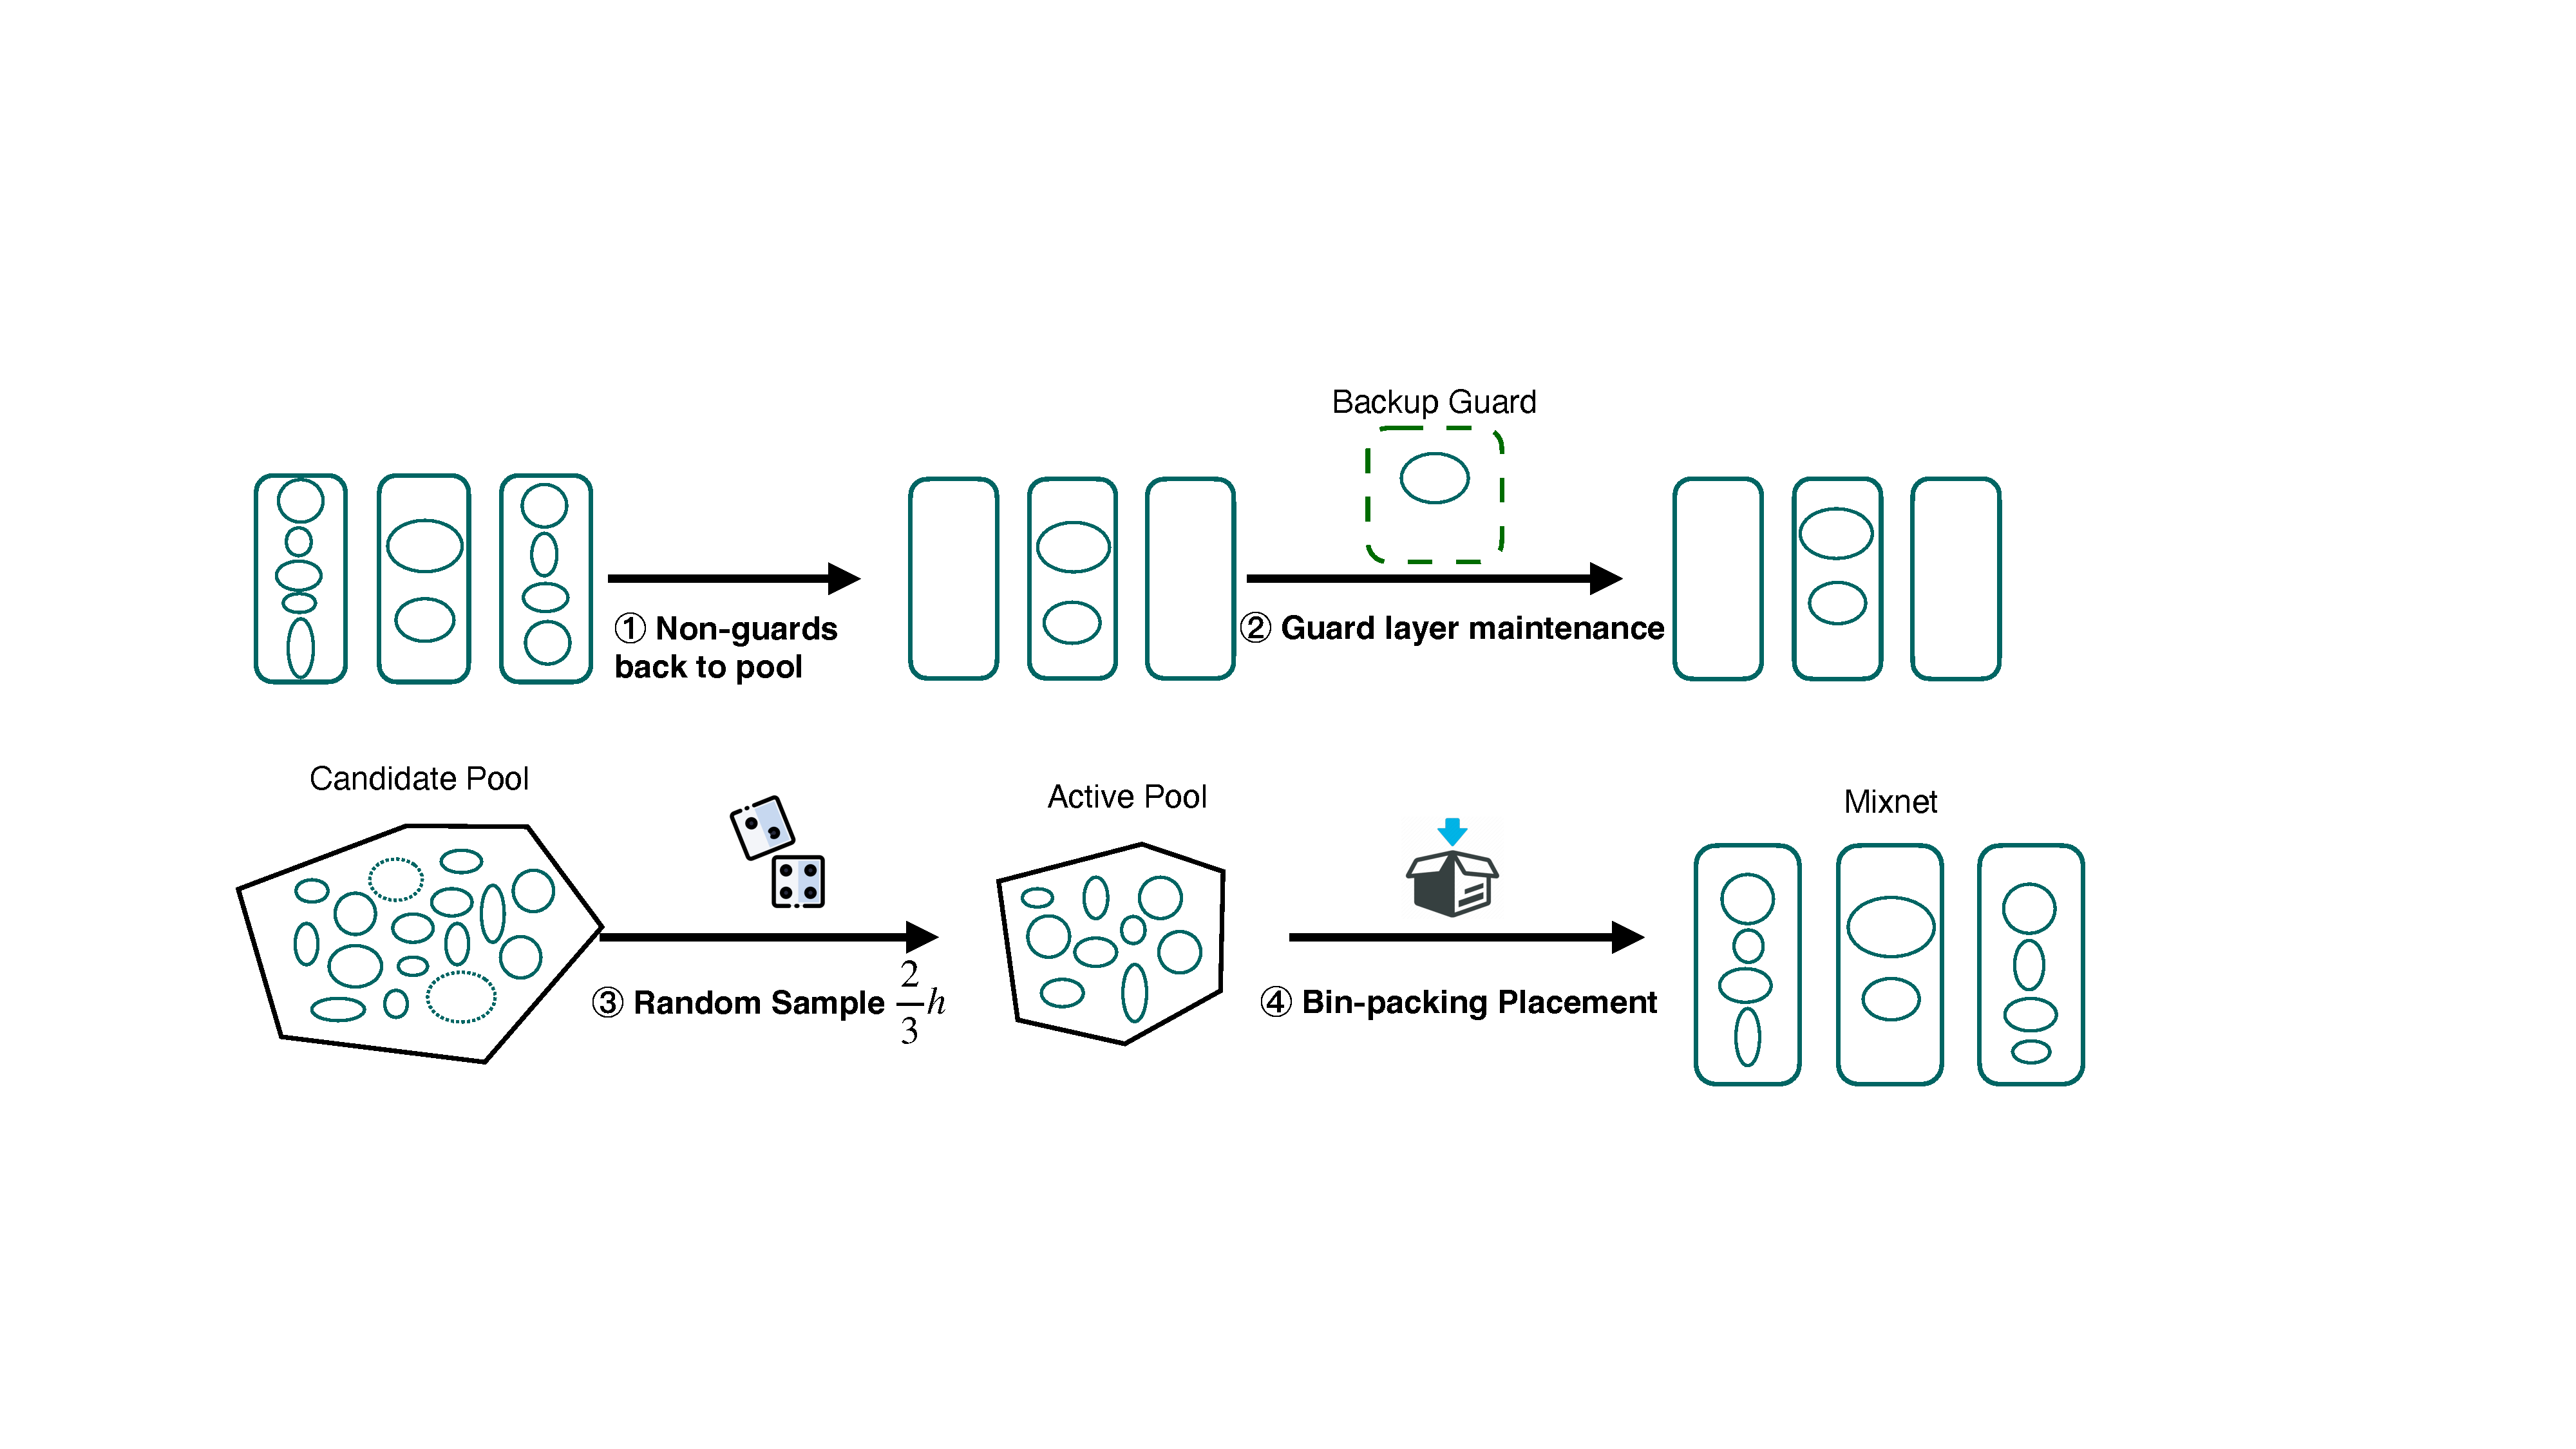
\includegraphics[width=0.95\rightcolwidth]{images/bowtie_maintain.pdf}
%    \caption{Mixnet Maintenance}
%    \end{figure}
    \vspace{0.5cm}
    \begin{figure}[t]
    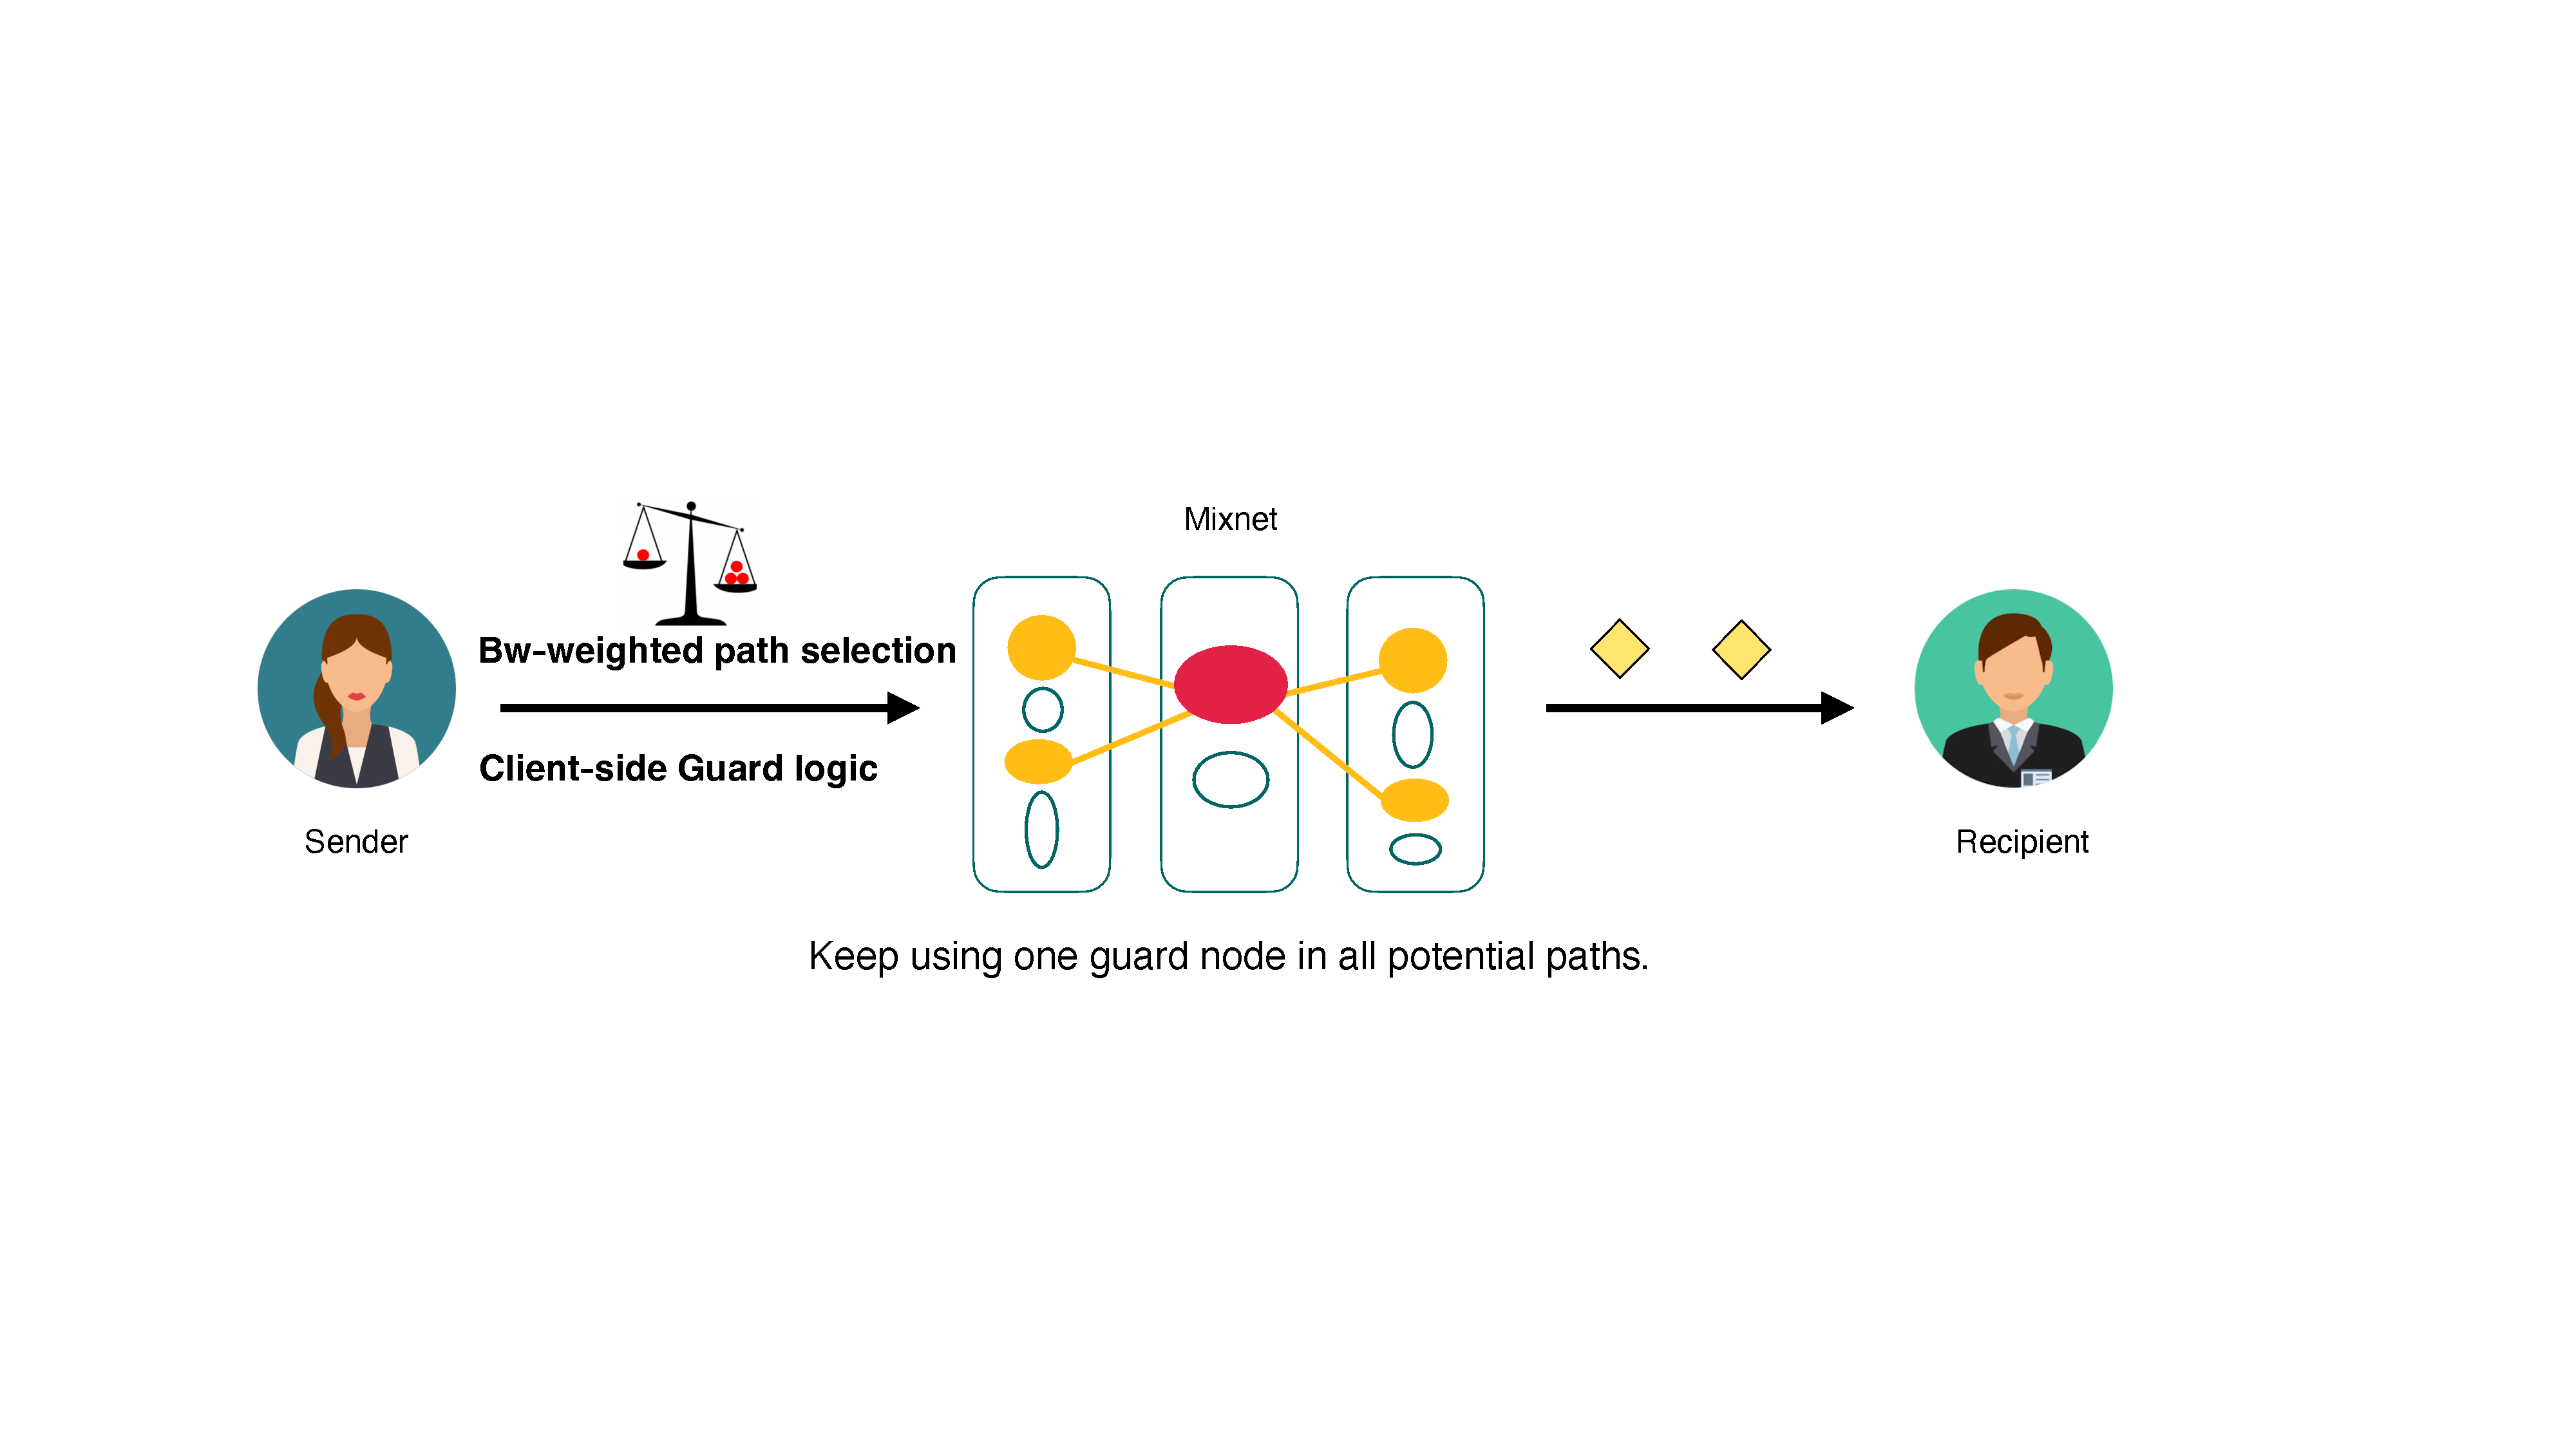
\includegraphics[width=0.95\rightcolwidth]{images/bowtie_routing.pdf}
    \caption{Mixnet Routing}
    \end{figure}
    \vspace{-1cm}
    \heading{Takeaways}
    \begin{itemize}
    \item A constrained guard layer that is populated with stable and high performant relays creates a challenge for the adversary.
    \item Bow-Tie finds a good balance between security and performance.
    \end{itemize}
  \end{block}


%  \begin{block}{Key Takeaways}
%    There have been a lot of exciting findings in this work, including key takeaways as follows:
%    \begin{itemize}
%      \item Bow-Tie provides higher level security than others presently; it enables good performance and efficiency as well.
%      %\item Bow-Tie balances the tradeoff between security and performance.
%      \item Using guards in layered routing for mixnets lowers the risk of users being de-anonymised.
%      \item Bandwidth-weighted path selection provides better load balance and security level.
%    \end{itemize}
%  \end{block}

\vspace{-1cm}
  \begin{block}{Contact}
  \begin{minipage}[t]{0.2\rightcolwidth}
  \end{minipage}
  \hfill
  \begin{minipage}[t]{0.3\rightcolwidth}
 \centering
    \textbf{x.ma@ed.ac.uk}\\
    \textbf{frochet@ed.ac.uk}\\
    \textbf{t.elahi@ed.ac.uk}
  \end{minipage}
  \hfil
  \begin{minipage}[t]{0.3\rightcolwidth}
  \vspace{-1cm}
  \begin{figure}
  
\includegraphics[width=0.5\textwidth]{images/artifact.png}
  \end{figure}
  \end{minipage}
  \hfill
  \begin{minipage}[t]{0.2\rightcolwidth}
  \end{minipage}

 
  \end{block}

 % \begin{figure}
      %
\includegraphics[scale=2]{images/logo.png}
  %\end{figure}
  %\begin{figure}
    %\includegraphics[scale=0.7]{images/innoviris-brussels-empowering-research.png}
  %\end{figure}

\end{column}

\separatorcolumn
\end{columns}
\end{frame}

\end{document}
